\documentclass[twoside]{book}

% Packages required by doxygen
\usepackage{fixltx2e}
\usepackage{calc}
\usepackage{doxygen}
\usepackage[export]{adjustbox} % also loads graphicx
\usepackage{graphicx}
\usepackage[utf8]{inputenc}
\usepackage{makeidx}
\usepackage{multicol}
\usepackage{multirow}
\PassOptionsToPackage{warn}{textcomp}
\usepackage{textcomp}
\usepackage[nointegrals]{wasysym}
\usepackage[table]{xcolor}

% Font selection
\usepackage[T1]{fontenc}
\usepackage[scaled=.90]{helvet}
\usepackage{courier}
\usepackage{amssymb}
\usepackage{sectsty}
\renewcommand{\familydefault}{\sfdefault}
\allsectionsfont{%
  \fontseries{bc}\selectfont%
  \color{darkgray}%
}
\renewcommand{\DoxyLabelFont}{%
  \fontseries{bc}\selectfont%
  \color{darkgray}%
}
\newcommand{\+}{\discretionary{\mbox{\scriptsize$\hookleftarrow$}}{}{}}

% Page & text layout
\usepackage{geometry}
\geometry{%
  a4paper,%
  top=2.5cm,%
  bottom=2.5cm,%
  left=2.5cm,%
  right=2.5cm%
}
\tolerance=750
\hfuzz=15pt
\hbadness=750
\setlength{\emergencystretch}{15pt}
\setlength{\parindent}{0cm}
\setlength{\parskip}{3ex plus 2ex minus 2ex}
\makeatletter
\renewcommand{\paragraph}{%
  \@startsection{paragraph}{4}{0ex}{-1.0ex}{1.0ex}{%
    \normalfont\normalsize\bfseries\SS@parafont%
  }%
}
\renewcommand{\subparagraph}{%
  \@startsection{subparagraph}{5}{0ex}{-1.0ex}{1.0ex}{%
    \normalfont\normalsize\bfseries\SS@subparafont%
  }%
}
\makeatother

% Headers & footers
\usepackage{fancyhdr}
\pagestyle{fancyplain}
\fancyhead[LE]{\fancyplain{}{\bfseries\thepage}}
\fancyhead[CE]{\fancyplain{}{}}
\fancyhead[RE]{\fancyplain{}{\bfseries\leftmark}}
\fancyhead[LO]{\fancyplain{}{\bfseries\rightmark}}
\fancyhead[CO]{\fancyplain{}{}}
\fancyhead[RO]{\fancyplain{}{\bfseries\thepage}}
\fancyfoot[LE]{\fancyplain{}{}}
\fancyfoot[CE]{\fancyplain{}{}}
\fancyfoot[RE]{\fancyplain{}{\bfseries\scriptsize Generated by Doxygen }}
\fancyfoot[LO]{\fancyplain{}{\bfseries\scriptsize Generated by Doxygen }}
\fancyfoot[CO]{\fancyplain{}{}}
\fancyfoot[RO]{\fancyplain{}{}}
\renewcommand{\footrulewidth}{0.4pt}
\renewcommand{\chaptermark}[1]{%
  \markboth{#1}{}%
}
\renewcommand{\sectionmark}[1]{%
  \markright{\thesection\ #1}%
}

% Indices & bibliography
\usepackage{natbib}
\usepackage[titles]{tocloft}
\setcounter{tocdepth}{3}
\setcounter{secnumdepth}{5}
\makeindex

% Hyperlinks (required, but should be loaded last)
\usepackage{ifpdf}
\ifpdf
  \usepackage[pdftex,pagebackref=true]{hyperref}
\else
  \usepackage[ps2pdf,pagebackref=true]{hyperref}
\fi
\hypersetup{%
  colorlinks=true,%
  linkcolor=blue,%
  citecolor=blue,%
  unicode%
}

% Custom commands
\newcommand{\clearemptydoublepage}{%
  \newpage{\pagestyle{empty}\cleardoublepage}%
}

\usepackage{caption}
\captionsetup{labelsep=space,justification=centering,font={bf},singlelinecheck=off,skip=4pt,position=top}

%===== C O N T E N T S =====

\begin{document}

% Titlepage & ToC
\hypersetup{pageanchor=false,
             bookmarksnumbered=true,
             pdfencoding=unicode
            }
\pagenumbering{roman}
\begin{titlepage}
\vspace*{7cm}
\begin{center}%
{\Large Face Verification for an Acess Control System }\\
\vspace*{1cm}
{\large Generated by Doxygen 1.8.11}\\
\end{center}
\end{titlepage}
\clearemptydoublepage
\tableofcontents
\clearemptydoublepage
\pagenumbering{arabic}
\hypersetup{pageanchor=true}

%--- Begin generated contents ---
\chapter{Namespace Index}
\section{Namespace List}
Here is a list of all documented namespaces with brief descriptions\-:\begin{DoxyCompactList}
\item\contentsline{section}{\hyperlink{namespaceauxiliary}{auxiliary} }{\pageref{namespaceauxiliary}}{}
\item\contentsline{section}{\hyperlink{namespacefacetracker}{facetracker} }{\pageref{namespacefacetracker}}{}
\item\contentsline{section}{\hyperlink{namespaceimg__screen}{img\-\_\-screen} }{\pageref{namespaceimg__screen}}{}
\item\contentsline{section}{\hyperlink{namespaceimg__screen__entry}{img\-\_\-screen\-\_\-entry} }{\pageref{namespaceimg__screen__entry}}{}
\item\contentsline{section}{\hyperlink{namespaceNFC__Arduino}{N\-F\-C\-\_\-\-Arduino} }{\pageref{namespaceNFC__Arduino}}{}
\item\contentsline{section}{\hyperlink{namespaceRecognitionFactory}{Recognition\-Factory} }{\pageref{namespaceRecognitionFactory}}{}
\item\contentsline{section}{\hyperlink{namespaceregister__facetracker}{register\-\_\-facetracker} }{\pageref{namespaceregister__facetracker}}{}
\item\contentsline{section}{\hyperlink{namespaceregister__server}{register\-\_\-server} }{\pageref{namespaceregister__server}}{}
\item\contentsline{section}{\hyperlink{namespacesend__socket}{send\-\_\-socket} }{\pageref{namespacesend__socket}}{}
\item\contentsline{section}{\hyperlink{namespaceverification__server}{verification\-\_\-server} }{\pageref{namespaceverification__server}}{}
\end{DoxyCompactList}

\chapter{Hierarchical Index}
\section{Class Hierarchy}
This inheritance list is sorted roughly, but not completely, alphabetically\-:\begin{DoxyCompactList}
\item \contentsline{section}{Calibration}{\pageref{classCalibration}}{}
\item \contentsline{section}{Camera}{\pageref{classCamera}}{}
\item object\begin{DoxyCompactList}
\item \contentsline{section}{Recognition\-Factory.\-Recognition\-Algorithm}{\pageref{classRecognitionFactory_1_1RecognitionAlgorithm}}{}
\begin{DoxyCompactList}
\item \contentsline{section}{Recognition\-Factory.\-d\-Lib}{\pageref{classRecognitionFactory_1_1dLib}}{}
\item \contentsline{section}{Recognition\-Factory.\-Open\-Face}{\pageref{classRecognitionFactory_1_1OpenFace}}{}
\end{DoxyCompactList}
\end{DoxyCompactList}
\end{DoxyCompactList}

\chapter{Class Index}
\section{Class List}
Here are the classes, structs, unions and interfaces with brief descriptions\+:\begin{DoxyCompactList}
\item\contentsline{section}{\hyperlink{classRecognitionFactory_1_1DeepFace}{Recognition\+Factory.\+Deep\+Face} }{\pageref{classRecognitionFactory_1_1DeepFace}}{}
\item\contentsline{section}{\hyperlink{classDetectionFactory_1_1DetectionAlgorithm}{Detection\+Factory.\+Detection\+Algorithm} }{\pageref{classDetectionFactory_1_1DetectionAlgorithm}}{}
\item\contentsline{section}{\hyperlink{classRecognitionFactory_1_1dLib}{Recognition\+Factory.\+d\+Lib} }{\pageref{classRecognitionFactory_1_1dLib}}{}
\item\contentsline{section}{\hyperlink{classDetectionFactory_1_1dLib}{Detection\+Factory.\+d\+Lib} }{\pageref{classDetectionFactory_1_1dLib}}{}
\item\contentsline{section}{\hyperlink{classfacenet_1_1ImageClass}{facenet.\+Image\+Class} }{\pageref{classfacenet_1_1ImageClass}}{}
\item\contentsline{section}{\hyperlink{classDetectionFactory_1_1MTCNN}{Detection\+Factory.\+M\+T\+C\+NN} }{\pageref{classDetectionFactory_1_1MTCNN}}{}
\item\contentsline{section}{\hyperlink{classdetect__face_1_1Network}{detect\+\_\+face.\+Network} }{\pageref{classdetect__face_1_1Network}}{}
\item\contentsline{section}{\hyperlink{classdetect__face_1_1ONet}{detect\+\_\+face.\+O\+Net} }{\pageref{classdetect__face_1_1ONet}}{}
\item\contentsline{section}{\hyperlink{classRecognitionFactory_1_1OpenFace}{Recognition\+Factory.\+Open\+Face} }{\pageref{classRecognitionFactory_1_1OpenFace}}{}
\item\contentsline{section}{\hyperlink{classdetect__face_1_1PNet}{detect\+\_\+face.\+P\+Net} }{\pageref{classdetect__face_1_1PNet}}{}
\item\contentsline{section}{\hyperlink{classRecognitionFactory_1_1RecognitionAlgorithm}{Recognition\+Factory.\+Recognition\+Algorithm} }{\pageref{classRecognitionFactory_1_1RecognitionAlgorithm}}{}
\item\contentsline{section}{\hyperlink{classdetect__face_1_1RNet}{detect\+\_\+face.\+R\+Net} }{\pageref{classdetect__face_1_1RNet}}{}
\end{DoxyCompactList}

\chapter{Namespace Documentation}
\hypertarget{namespacedetect__face}{}\section{detect\+\_\+face Namespace Reference}
\label{namespacedetect__face}\index{detect\+\_\+face@{detect\+\_\+face}}
\subsection*{Classes}
\begin{DoxyCompactItemize}
\item 
class \hyperlink{classdetect__face_1_1Network}{Network}
\item 
class \hyperlink{classdetect__face_1_1ONet}{O\+Net}
\item 
class \hyperlink{classdetect__face_1_1PNet}{P\+Net}
\item 
class \hyperlink{classdetect__face_1_1RNet}{R\+Net}
\end{DoxyCompactItemize}
\subsection*{Functions}
\begin{DoxyCompactItemize}
\item 
def \hyperlink{namespacedetect__face_a56206197555d7b54d5f27c410d814268}{layer} (op)
\item 
def {\bfseries create\+\_\+mtcnn} (sess, model\+\_\+path)\hypertarget{namespacedetect__face_a9a159b63bb8dfd9836c1a5a401d82acc}{}\label{namespacedetect__face_a9a159b63bb8dfd9836c1a5a401d82acc}

\item 
def {\bfseries detect\+\_\+face} (img, minsize, pnet, rnet, onet, threshold, factor)\hypertarget{namespacedetect__face_a114ff784601bf295b09cbda8e43c1f40}{}\label{namespacedetect__face_a114ff784601bf295b09cbda8e43c1f40}

\item 
def {\bfseries bulk\+\_\+detect\+\_\+face} (images, detection\+\_\+window\+\_\+size\+\_\+ratio, pnet, rnet, onet, threshold, factor)\hypertarget{namespacedetect__face_a03662ace7b5ad080897d8fad2213e2ea}{}\label{namespacedetect__face_a03662ace7b5ad080897d8fad2213e2ea}

\item 
def {\bfseries bbreg} (boundingbox, reg)\hypertarget{namespacedetect__face_a8d2a300cd87264905d5edd788c4d1a35}{}\label{namespacedetect__face_a8d2a300cd87264905d5edd788c4d1a35}

\item 
def {\bfseries generate\+Bounding\+Box} (imap, reg, scale, t)\hypertarget{namespacedetect__face_a1fd06dbdc98718c9e9e05636c22864ce}{}\label{namespacedetect__face_a1fd06dbdc98718c9e9e05636c22864ce}

\item 
def {\bfseries nms} (boxes, threshold, method)\hypertarget{namespacedetect__face_a2e44d4e2710d931d974bbfc4237e5964}{}\label{namespacedetect__face_a2e44d4e2710d931d974bbfc4237e5964}

\item 
def {\bfseries pad} (total\+\_\+boxes, w, h)\hypertarget{namespacedetect__face_adb76cb941cd3edc02296995e3d0759ca}{}\label{namespacedetect__face_adb76cb941cd3edc02296995e3d0759ca}

\item 
def {\bfseries rerec} (bboxA)\hypertarget{namespacedetect__face_acfe26effdb21d6424211964e67974e2c}{}\label{namespacedetect__face_acfe26effdb21d6424211964e67974e2c}

\item 
def {\bfseries imresample} (img, sz)\hypertarget{namespacedetect__face_ad0751aa76758f14c208ff91a53a90b9a}{}\label{namespacedetect__face_ad0751aa76758f14c208ff91a53a90b9a}

\end{DoxyCompactItemize}


\subsection{Detailed Description}
\begin{DoxyVerb}Tensorflow implementation of the face detection / alignment algorithm found at
https://github.com/kpzhang93/MTCNN_face_detection_alignment
\end{DoxyVerb}
 

\subsection{Function Documentation}
\index{detect\+\_\+face@{detect\+\_\+face}!layer@{layer}}
\index{layer@{layer}!detect\+\_\+face@{detect\+\_\+face}}
\subsubsection[{\texorpdfstring{layer(op)}{layer(op)}}]{\setlength{\rightskip}{0pt plus 5cm}def detect\+\_\+face.\+layer (
\begin{DoxyParamCaption}
\item[{}]{op}
\end{DoxyParamCaption}
)}\hypertarget{namespacedetect__face_a56206197555d7b54d5f27c410d814268}{}\label{namespacedetect__face_a56206197555d7b54d5f27c410d814268}
\begin{DoxyVerb}Decorator for composable network layers.\end{DoxyVerb}
 
\hypertarget{namespacefacenet}{}\section{facenet Namespace Reference}
\label{namespacefacenet}\index{facenet@{facenet}}
\subsection*{Classes}
\begin{DoxyCompactItemize}
\item 
class \hyperlink{classfacenet_1_1ImageClass}{Image\+Class}
\end{DoxyCompactItemize}
\subsection*{Functions}
\begin{DoxyCompactItemize}
\item 
def \hyperlink{namespacefacenet_a8687a4b833d739733305b1df325fb888}{triplet\+\_\+loss} (anchor, positive, negative, alpha)
\item 
def \hyperlink{namespacefacenet_ab63b951bab1032f33280607a4d099c2c}{decov\+\_\+loss} (xs)
\item 
def \hyperlink{namespacefacenet_ac610e0e8e066018e8abb4229542cfca3}{center\+\_\+loss} (features, label, alfa, nrof\+\_\+classes)
\item 
def {\bfseries get\+\_\+image\+\_\+paths\+\_\+and\+\_\+labels} (dataset)\hypertarget{namespacefacenet_a722a386f9002e327c8bed3ac2cbf0e83}{}\label{namespacefacenet_a722a386f9002e327c8bed3ac2cbf0e83}

\item 
def {\bfseries shuffle\+\_\+examples} (image\+\_\+paths, labels)\hypertarget{namespacefacenet_adad57c35372b07640d9b728e7586d273}{}\label{namespacefacenet_adad57c35372b07640d9b728e7586d273}

\item 
def \hyperlink{namespacefacenet_ab468887342368153445c951db5cebb69}{read\+\_\+images\+\_\+from\+\_\+disk} (input\+\_\+queue)
\item 
def {\bfseries random\+\_\+rotate\+\_\+image} (image)\hypertarget{namespacefacenet_ab44fa62068a1e719d931091e5f616c17}{}\label{namespacefacenet_ab44fa62068a1e719d931091e5f616c17}

\item 
def {\bfseries read\+\_\+and\+\_\+augment\+\_\+data} (image\+\_\+list, label\+\_\+list, image\+\_\+size, batch\+\_\+size, max\+\_\+nrof\+\_\+epochs, random\+\_\+crop, random\+\_\+flip, random\+\_\+rotate, nrof\+\_\+preprocess\+\_\+threads, shuffle=True)\hypertarget{namespacefacenet_a3cffda165223d8823bc4c2854b715b96}{}\label{namespacefacenet_a3cffda165223d8823bc4c2854b715b96}

\item 
def {\bfseries train} (total\+\_\+loss, global\+\_\+step, optimizer, learning\+\_\+rate, moving\+\_\+average\+\_\+decay, update\+\_\+gradient\+\_\+vars, log\+\_\+histograms=True)\hypertarget{namespacefacenet_acd1a15c58c23e784fb0fe17dfb63a3e7}{}\label{namespacefacenet_acd1a15c58c23e784fb0fe17dfb63a3e7}

\item 
def {\bfseries prewhiten} (x)\hypertarget{namespacefacenet_ae59f1f702cf24ee44e1cbc87c040ba9f}{}\label{namespacefacenet_ae59f1f702cf24ee44e1cbc87c040ba9f}

\item 
def {\bfseries crop} (image, random\+\_\+crop, image\+\_\+size)\hypertarget{namespacefacenet_a566cf422af34d218be5bece0dd3cc3bf}{}\label{namespacefacenet_a566cf422af34d218be5bece0dd3cc3bf}

\item 
def {\bfseries flip} (image, random\+\_\+flip)\hypertarget{namespacefacenet_aabe975dd0bab8526f1801793a802357f}{}\label{namespacefacenet_aabe975dd0bab8526f1801793a802357f}

\item 
def {\bfseries to\+\_\+rgb} (img)\hypertarget{namespacefacenet_ad4660d94910e620f360b6218736856dc}{}\label{namespacefacenet_ad4660d94910e620f360b6218736856dc}

\item 
def {\bfseries load\+\_\+data} (image\+\_\+paths, do\+\_\+random\+\_\+crop, do\+\_\+random\+\_\+flip, image\+\_\+size, do\+\_\+prewhiten=True)\hypertarget{namespacefacenet_ab514bbfd01b3545290e35c84ee1811e0}{}\label{namespacefacenet_ab514bbfd01b3545290e35c84ee1811e0}

\item 
def {\bfseries get\+\_\+label\+\_\+batch} (label\+\_\+data, batch\+\_\+size, batch\+\_\+index)\hypertarget{namespacefacenet_a66df4716495582a9c75e6a25730b5123}{}\label{namespacefacenet_a66df4716495582a9c75e6a25730b5123}

\item 
def {\bfseries get\+\_\+batch} (image\+\_\+data, batch\+\_\+size, batch\+\_\+index)\hypertarget{namespacefacenet_a39defc57ede0e7947ff03649bc25731a}{}\label{namespacefacenet_a39defc57ede0e7947ff03649bc25731a}

\item 
def {\bfseries get\+\_\+triplet\+\_\+batch} (triplets, batch\+\_\+index, batch\+\_\+size)\hypertarget{namespacefacenet_ad8699592011faac256ff18738d72625c}{}\label{namespacefacenet_ad8699592011faac256ff18738d72625c}

\item 
def {\bfseries get\+\_\+learning\+\_\+rate\+\_\+from\+\_\+file} (filename, epoch)\hypertarget{namespacefacenet_a3575f9424fa72db6e13fed9533e6f082}{}\label{namespacefacenet_a3575f9424fa72db6e13fed9533e6f082}

\item 
def {\bfseries get\+\_\+dataset} (paths, has\+\_\+class\+\_\+directories=True)\hypertarget{namespacefacenet_a4e5a7e85a4d83056dd83906c2be7e6cd}{}\label{namespacefacenet_a4e5a7e85a4d83056dd83906c2be7e6cd}

\item 
def {\bfseries get\+\_\+image\+\_\+paths} (facedir)\hypertarget{namespacefacenet_aaea60084eb6a8fa08d2916328fc31445}{}\label{namespacefacenet_aaea60084eb6a8fa08d2916328fc31445}

\item 
def {\bfseries split\+\_\+dataset} (dataset, split\+\_\+ratio, mode)\hypertarget{namespacefacenet_a9c02e7ae77e659339c1dfdad52bb9672}{}\label{namespacefacenet_a9c02e7ae77e659339c1dfdad52bb9672}

\item 
def {\bfseries load\+\_\+model} (model)\hypertarget{namespacefacenet_aa5f45188071fba9ce085778952aa238a}{}\label{namespacefacenet_aa5f45188071fba9ce085778952aa238a}

\item 
def {\bfseries get\+\_\+model\+\_\+filenames} (model\+\_\+dir)\hypertarget{namespacefacenet_a088d111a6a03d2c39e70ffb4cf0cedd0}{}\label{namespacefacenet_a088d111a6a03d2c39e70ffb4cf0cedd0}

\item 
def {\bfseries calculate\+\_\+roc} (thresholds, embeddings1, embeddings2, actual\+\_\+issame, nrof\+\_\+folds=10)\hypertarget{namespacefacenet_a9d781a188f85b866a3a0b854bf42de45}{}\label{namespacefacenet_a9d781a188f85b866a3a0b854bf42de45}

\item 
def {\bfseries calculate\+\_\+accuracy} (threshold, dist, actual\+\_\+issame)\hypertarget{namespacefacenet_ab94a07008ed9a2aaabe8779d11652971}{}\label{namespacefacenet_ab94a07008ed9a2aaabe8779d11652971}

\item 
def {\bfseries calculate\+\_\+val} (thresholds, embeddings1, embeddings2, actual\+\_\+issame, far\+\_\+target, nrof\+\_\+folds=10)\hypertarget{namespacefacenet_a891847781d812f6922c60e44cea7e27f}{}\label{namespacefacenet_a891847781d812f6922c60e44cea7e27f}

\item 
def {\bfseries calculate\+\_\+val\+\_\+far} (threshold, dist, actual\+\_\+issame)\hypertarget{namespacefacenet_ac50c9595f2c719fd93f5bb8c6568da23}{}\label{namespacefacenet_ac50c9595f2c719fd93f5bb8c6568da23}

\item 
def {\bfseries store\+\_\+revision\+\_\+info} (src\+\_\+path, output\+\_\+dir, arg\+\_\+string)\hypertarget{namespacefacenet_afd1075cd7525c57f5c9071a49b13332d}{}\label{namespacefacenet_afd1075cd7525c57f5c9071a49b13332d}

\item 
def {\bfseries list\+\_\+variables} (filename)\hypertarget{namespacefacenet_a5d6490a85f6bc56f3e5da8ef56b0c378}{}\label{namespacefacenet_a5d6490a85f6bc56f3e5da8ef56b0c378}

\item 
def {\bfseries put\+\_\+images\+\_\+on\+\_\+grid} (images, shape=(16, 8))\hypertarget{namespacefacenet_a7be95084243b7d886cd39799179d199f}{}\label{namespacefacenet_a7be95084243b7d886cd39799179d199f}

\item 
def {\bfseries write\+\_\+arguments\+\_\+to\+\_\+file} (args, filename)\hypertarget{namespacefacenet_aeff6337261a1c0dbb1a9b1a502f0f358}{}\label{namespacefacenet_aeff6337261a1c0dbb1a9b1a502f0f358}

\end{DoxyCompactItemize}


\subsection{Detailed Description}
\begin{DoxyVerb}Functions for building the face recognition network.
\end{DoxyVerb}
 

\subsection{Function Documentation}
\index{facenet@{facenet}!center\+\_\+loss@{center\+\_\+loss}}
\index{center\+\_\+loss@{center\+\_\+loss}!facenet@{facenet}}
\subsubsection[{\texorpdfstring{center\+\_\+loss(features, label, alfa, nrof\+\_\+classes)}{center_loss(features, label, alfa, nrof_classes)}}]{\setlength{\rightskip}{0pt plus 5cm}def facenet.\+center\+\_\+loss (
\begin{DoxyParamCaption}
\item[{}]{features, }
\item[{}]{label, }
\item[{}]{alfa, }
\item[{}]{nrof\+\_\+classes}
\end{DoxyParamCaption}
)}\hypertarget{namespacefacenet_ac610e0e8e066018e8abb4229542cfca3}{}\label{namespacefacenet_ac610e0e8e066018e8abb4229542cfca3}
\begin{DoxyVerb}Center loss based on the paper "A Discriminative Feature Learning Approach for Deep Face Recognition"
   (http://ydwen.github.io/papers/WenECCV16.pdf)
\end{DoxyVerb}
 \index{facenet@{facenet}!decov\+\_\+loss@{decov\+\_\+loss}}
\index{decov\+\_\+loss@{decov\+\_\+loss}!facenet@{facenet}}
\subsubsection[{\texorpdfstring{decov\+\_\+loss(xs)}{decov_loss(xs)}}]{\setlength{\rightskip}{0pt plus 5cm}def facenet.\+decov\+\_\+loss (
\begin{DoxyParamCaption}
\item[{}]{xs}
\end{DoxyParamCaption}
)}\hypertarget{namespacefacenet_ab63b951bab1032f33280607a4d099c2c}{}\label{namespacefacenet_ab63b951bab1032f33280607a4d099c2c}
\begin{DoxyVerb}Decov loss as described in https://arxiv.org/pdf/1511.06068.pdf
'Reducing Overfitting In Deep Networks by Decorrelating Representation'
\end{DoxyVerb}
 \index{facenet@{facenet}!read\+\_\+images\+\_\+from\+\_\+disk@{read\+\_\+images\+\_\+from\+\_\+disk}}
\index{read\+\_\+images\+\_\+from\+\_\+disk@{read\+\_\+images\+\_\+from\+\_\+disk}!facenet@{facenet}}
\subsubsection[{\texorpdfstring{read\+\_\+images\+\_\+from\+\_\+disk(input\+\_\+queue)}{read_images_from_disk(input_queue)}}]{\setlength{\rightskip}{0pt plus 5cm}def facenet.\+read\+\_\+images\+\_\+from\+\_\+disk (
\begin{DoxyParamCaption}
\item[{}]{input\+\_\+queue}
\end{DoxyParamCaption}
)}\hypertarget{namespacefacenet_ab468887342368153445c951db5cebb69}{}\label{namespacefacenet_ab468887342368153445c951db5cebb69}
\begin{DoxyVerb}Consumes a single filename and label as a ' '-delimited string.
Args:
  filename_and_label_tensor: A scalar string tensor.
Returns:
  Two tensors: the decoded image, and the string label.
\end{DoxyVerb}
 \index{facenet@{facenet}!triplet\+\_\+loss@{triplet\+\_\+loss}}
\index{triplet\+\_\+loss@{triplet\+\_\+loss}!facenet@{facenet}}
\subsubsection[{\texorpdfstring{triplet\+\_\+loss(anchor, positive, negative, alpha)}{triplet_loss(anchor, positive, negative, alpha)}}]{\setlength{\rightskip}{0pt plus 5cm}def facenet.\+triplet\+\_\+loss (
\begin{DoxyParamCaption}
\item[{}]{anchor, }
\item[{}]{positive, }
\item[{}]{negative, }
\item[{}]{alpha}
\end{DoxyParamCaption}
)}\hypertarget{namespacefacenet_a8687a4b833d739733305b1df325fb888}{}\label{namespacefacenet_a8687a4b833d739733305b1df325fb888}
\begin{DoxyVerb}Calculate the triplet loss according to the FaceNet paper

Args:
  anchor: the embeddings for the anchor images.
  positive: the embeddings for the positive images.
  negative: the embeddings for the negative images.
  
Returns:
  the triplet loss according to the FaceNet paper as a float tensor.
\end{DoxyVerb}
 
\hypertarget{namespacefacetracker}{\section{facetracker Namespace Reference}
\label{namespacefacetracker}\index{facetracker@{facetracker}}
}
\subsection*{Functions}
\begin{DoxyCompactItemize}
\item 
def \hyperlink{namespacefacetracker_afd03f1d703bca2c3f01ceac6ca711f17}{recvall}
\begin{DoxyCompactList}\small\item\em Function that will convert the socket received into a string. \end{DoxyCompactList}\item 
\hypertarget{namespacefacetracker_a8c68f7ebd8f2b1e99b6d3336430ad2be}{def {\bfseries main}}\label{namespacefacetracker_a8c68f7ebd8f2b1e99b6d3336430ad2be}

\end{DoxyCompactItemize}
\subsection*{Variables}
\begin{DoxyCompactItemize}
\item 
\hypertarget{namespacefacetracker_af8f8c0f83a1bcab62b58ffe151d54257}{{\bfseries font} = cv2.\-F\-O\-N\-T\-\_\-\-H\-E\-R\-S\-H\-E\-Y\-\_\-\-S\-I\-M\-P\-L\-E\-X}\label{namespacefacetracker_af8f8c0f83a1bcab62b58ffe151d54257}

\item 
\hypertarget{namespacefacetracker_a0d3f577882e0f8deade5722e75594b58}{string {\bfseries T\-C\-P\-\_\-\-I\-P} = 'localhost'}\label{namespacefacetracker_a0d3f577882e0f8deade5722e75594b58}

\item 
\hypertarget{namespacefacetracker_a7fd84c2f2afecb14acb6526007adb04a}{int {\bfseries T\-C\-P\-\_\-\-P\-O\-R\-T} = 8002}\label{namespacefacetracker_a7fd84c2f2afecb14acb6526007adb04a}

\end{DoxyCompactItemize}


\subsection{Detailed Description}
\begin{DoxyVerb}Program that tracks the face of the subject that appears on the camera for the verification process (turnstile simulation). 
It will also calulate the descriptors that define the face presented and, if needed, it will send such descriptors to the verification server.
Finally, the program will send a signal to the camera acquisition program if the person changes for a further calibration. 
\end{DoxyVerb}
 

\subsection{Function Documentation}
\hypertarget{namespacefacetracker_afd03f1d703bca2c3f01ceac6ca711f17}{\index{facetracker@{facetracker}!recvall@{recvall}}
\index{recvall@{recvall}!facetracker@{facetracker}}
\subsubsection[{recvall}]{\setlength{\rightskip}{0pt plus 5cm}def facetracker.\-recvall (
\begin{DoxyParamCaption}
\item[{}]{sock, }
\item[{}]{count}
\end{DoxyParamCaption}
)}}\label{namespacefacetracker_afd03f1d703bca2c3f01ceac6ca711f17}


Function that will convert the socket received into a string. 


\begin{DoxyParams}{Parameters}
{\em sock} & The socket \\
\hline
{\em count} & The socket size\\
\hline
\end{DoxyParams}
String Socket Information 
\hypertarget{namespaceimg__screen}{}\section{img\+\_\+screen Namespace Reference}
\label{namespaceimg__screen}\index{img\+\_\+screen@{img\+\_\+screen}}
\subsection*{Functions}
\begin{DoxyCompactItemize}
\item 
def \hyperlink{namespaceimg__screen_acd79c234758f2fce61010e92079132f0}{recvall} (sock, count)
\begin{DoxyCompactList}\small\item\em Function that will convert the socket received into a string. \end{DoxyCompactList}\item 
def {\bfseries main} ()\hypertarget{namespaceimg__screen_a8b8effa7bd8a1c4faa77a39336eabdd4}{}\label{namespaceimg__screen_a8b8effa7bd8a1c4faa77a39336eabdd4}

\end{DoxyCompactItemize}
\subsection*{Variables}
\begin{DoxyCompactItemize}
\item 
string {\bfseries T\+C\+P\+\_\+\+IP} = \textquotesingle{}localhost\textquotesingle{}\hypertarget{namespaceimg__screen_a4ff0562588b8f821d56dc8c337a8002f}{}\label{namespaceimg__screen_a4ff0562588b8f821d56dc8c337a8002f}

\item 
int {\bfseries T\+C\+P\+\_\+\+P\+O\+RT} = 8004\hypertarget{namespaceimg__screen_abb1cc73fc386a79c181d62ea05038068}{}\label{namespaceimg__screen_abb1cc73fc386a79c181d62ea05038068}

\end{DoxyCompactItemize}


\subsection{Detailed Description}
\begin{DoxyVerb}Program that will present a full-screen image according to the signal received by the verification server.
\end{DoxyVerb}
 

\subsection{Function Documentation}
\index{img\+\_\+screen@{img\+\_\+screen}!recvall@{recvall}}
\index{recvall@{recvall}!img\+\_\+screen@{img\+\_\+screen}}
\subsubsection[{\texorpdfstring{recvall(sock, count)}{recvall(sock, count)}}]{\setlength{\rightskip}{0pt plus 5cm}def img\+\_\+screen.\+recvall (
\begin{DoxyParamCaption}
\item[{}]{sock, }
\item[{}]{count}
\end{DoxyParamCaption}
)}\hypertarget{namespaceimg__screen_acd79c234758f2fce61010e92079132f0}{}\label{namespaceimg__screen_acd79c234758f2fce61010e92079132f0}


Function that will convert the socket received into a string. 


\begin{DoxyParams}{Parameters}
{\em sock} & The socket \\
\hline
{\em count} & The socket size\\
\hline
\end{DoxyParams}
String Socket Information 
\hypertarget{namespaceimg__screen__entry}{\section{img\-\_\-screen\-\_\-entry Namespace Reference}
\label{namespaceimg__screen__entry}\index{img\-\_\-screen\-\_\-entry@{img\-\_\-screen\-\_\-entry}}
}
\subsection*{Functions}
\begin{DoxyCompactItemize}
\item 
def \hyperlink{namespaceimg__screen__entry_abf84aa8b7196bf3b6a61f59f66e518e4}{recvall}
\begin{DoxyCompactList}\small\item\em Function that will convert the socket received into a string. \end{DoxyCompactList}\item 
\hypertarget{namespaceimg__screen__entry_af37653694e0c32c14afbf6a49a08c9cf}{def {\bfseries main}}\label{namespaceimg__screen__entry_af37653694e0c32c14afbf6a49a08c9cf}

\end{DoxyCompactItemize}
\subsection*{Variables}
\begin{DoxyCompactItemize}
\item 
\hypertarget{namespaceimg__screen__entry_afe06b4e41a1facc65c4045482aaa4381}{string {\bfseries T\-C\-P\-\_\-\-I\-P} = 'localhost'}\label{namespaceimg__screen__entry_afe06b4e41a1facc65c4045482aaa4381}

\item 
\hypertarget{namespaceimg__screen__entry_acbc1d6aba5755d61c20444435e1b2934}{int {\bfseries T\-C\-P\-\_\-\-P\-O\-R\-T} = 8004}\label{namespaceimg__screen__entry_acbc1d6aba5755d61c20444435e1b2934}

\end{DoxyCompactItemize}


\subsection{Detailed Description}
\begin{DoxyVerb}Program that will present a full-screen image according to the signal received by the verification server.
\end{DoxyVerb}
 

\subsection{Function Documentation}
\hypertarget{namespaceimg__screen__entry_abf84aa8b7196bf3b6a61f59f66e518e4}{\index{img\-\_\-screen\-\_\-entry@{img\-\_\-screen\-\_\-entry}!recvall@{recvall}}
\index{recvall@{recvall}!img_screen_entry@{img\-\_\-screen\-\_\-entry}}
\subsubsection[{recvall}]{\setlength{\rightskip}{0pt plus 5cm}def img\-\_\-screen\-\_\-entry.\-recvall (
\begin{DoxyParamCaption}
\item[{}]{sock, }
\item[{}]{count}
\end{DoxyParamCaption}
)}}\label{namespaceimg__screen__entry_abf84aa8b7196bf3b6a61f59f66e518e4}


Function that will convert the socket received into a string. 


\begin{DoxyParams}{Parameters}
{\em sock} & The socket \\
\hline
{\em count} & The socket size\\
\hline
\end{DoxyParams}
String Socket Information 
\hypertarget{namespaceNFC__Arduino}{}\section{N\+F\+C\+\_\+\+Arduino Namespace Reference}
\label{namespaceNFC__Arduino}\index{N\+F\+C\+\_\+\+Arduino@{N\+F\+C\+\_\+\+Arduino}}
\subsection*{Variables}
\begin{DoxyCompactItemize}
\item 
{\bfseries ser} = serial.\+Serial(\textquotesingle{}/dev/tty\+U\+S\+B0\textquotesingle{}, 9600)\hypertarget{namespaceNFC__Arduino_a098df137056dd8f9401fc6ef83860406}{}\label{namespaceNFC__Arduino_a098df137056dd8f9401fc6ef83860406}

\item 
{\bfseries file} = open(\char`\"{}../../logs/logins.\+txt\char`\"{}, \char`\"{}a\char`\"{})\hypertarget{namespaceNFC__Arduino_acb7751cf964ffc03e1d78e06be636342}{}\label{namespaceNFC__Arduino_acb7751cf964ffc03e1d78e06be636342}

\item 
{\bfseries orig\+\_\+settings} = termios.\+tcgetattr(sys.\+stdin)\hypertarget{namespaceNFC__Arduino_afe70bff8432edcf8b18a189291eaff07}{}\label{namespaceNFC__Arduino_afe70bff8432edcf8b18a189291eaff07}

\item 
{\bfseries x} = None\hypertarget{namespaceNFC__Arduino_ae79f4584094541969c8ffe997d8e5a85}{}\label{namespaceNFC__Arduino_ae79f4584094541969c8ffe997d8e5a85}

\item 
{\bfseries stra} = ser.\+readline()\mbox{[}1\+:-\/2\mbox{]}\hypertarget{namespaceNFC__Arduino_a0f727b9d3472b437ae591c225f0bf456}{}\label{namespaceNFC__Arduino_a0f727b9d3472b437ae591c225f0bf456}

\end{DoxyCompactItemize}


\subsection{Detailed Description}
\begin{DoxyVerb}Program that it is used for read an Arduino connected on ttyUSB0 port which consequently has a RC522 NFC Reader connected to it.
Once a NFC value is read, it will send the hexadecimal value associated to the NFC Tag via socket. 
If the Arduino is not connected, the NFC ID can be simulated by a key from the keyboard.
\end{DoxyVerb}
 
\hypertarget{namespaceregister__facetracker}{}\section{register\+\_\+facetracker Namespace Reference}
\label{namespaceregister__facetracker}\index{register\+\_\+facetracker@{register\+\_\+facetracker}}
\subsection*{Functions}
\begin{DoxyCompactItemize}
\item 
def \hyperlink{namespaceregister__facetracker_a7e7317697e2ec6c09ed19d2be249da48}{recvall} (sock, count)
\begin{DoxyCompactList}\small\item\em Function that will convert the socket received into a string. \end{DoxyCompactList}\item 
def {\bfseries main} ()\hypertarget{namespaceregister__facetracker_a2020aecd0ed90359b49d4f16e5b469c9}{}\label{namespaceregister__facetracker_a2020aecd0ed90359b49d4f16e5b469c9}

\end{DoxyCompactItemize}
\subsection*{Variables}
\begin{DoxyCompactItemize}
\item 
{\bfseries font} = cv2.\+F\+O\+N\+T\+\_\+\+H\+E\+R\+S\+H\+E\+Y\+\_\+\+S\+I\+M\+P\+L\+EX\hypertarget{namespaceregister__facetracker_a40fd762d6e26811e038be5b5eabb4aef}{}\label{namespaceregister__facetracker_a40fd762d6e26811e038be5b5eabb4aef}

\item 
string {\bfseries T\+C\+P\+\_\+\+IP} = \textquotesingle{}localhost\textquotesingle{}\hypertarget{namespaceregister__facetracker_a8d029fb157738c48373876bb27ac948a}{}\label{namespaceregister__facetracker_a8d029fb157738c48373876bb27ac948a}

\item 
int {\bfseries T\+C\+P\+\_\+\+P\+O\+RT} = 8002\hypertarget{namespaceregister__facetracker_aff2158cc5bc813254a9b6253552907f7}{}\label{namespaceregister__facetracker_aff2158cc5bc813254a9b6253552907f7}

\item 
{\bfseries file} = open(\char`\"{}../../logs/registration\+\_\+values.\+txt\char`\"{}, \char`\"{}a\char`\"{})\hypertarget{namespaceregister__facetracker_a89f807184e61b9d93eef7c2c0a034fdc}{}\label{namespaceregister__facetracker_a89f807184e61b9d93eef7c2c0a034fdc}

\end{DoxyCompactItemize}


\subsection{Detailed Description}
\begin{DoxyVerb}Program that tracks the face of the subject that appears on the camera for the registration process (ticketline simulation). 
It will also calulate the descriptors that define the face presented and, if needed, it will send such descriptors to the verification server.
Finally, the program will send a signal to the camera acquisition program if the person changes for a further calibration. 
\end{DoxyVerb}
 

\subsection{Function Documentation}
\index{register\+\_\+facetracker@{register\+\_\+facetracker}!recvall@{recvall}}
\index{recvall@{recvall}!register\+\_\+facetracker@{register\+\_\+facetracker}}
\subsubsection[{\texorpdfstring{recvall(sock, count)}{recvall(sock, count)}}]{\setlength{\rightskip}{0pt plus 5cm}def register\+\_\+facetracker.\+recvall (
\begin{DoxyParamCaption}
\item[{}]{sock, }
\item[{}]{count}
\end{DoxyParamCaption}
)}\hypertarget{namespaceregister__facetracker_a7e7317697e2ec6c09ed19d2be249da48}{}\label{namespaceregister__facetracker_a7e7317697e2ec6c09ed19d2be249da48}


Function that will convert the socket received into a string. 


\begin{DoxyParams}{Parameters}
{\em sock} & The socket \\
\hline
{\em count} & The socket size\\
\hline
\end{DoxyParams}
String Socket Information 
\hypertarget{namespaceregister__server}{}\section{register\+\_\+server Namespace Reference}
\label{namespaceregister__server}\index{register\+\_\+server@{register\+\_\+server}}
\subsection*{Functions}
\begin{DoxyCompactItemize}
\item 
def \hyperlink{namespaceregister__server_a67bb86c0ff90fdf0fd4c77fa7eeeb1c1}{recvall} (sock, count)
\begin{DoxyCompactList}\small\item\em Function that will convert the socket received into a string. \end{DoxyCompactList}\item 
def \hyperlink{namespaceregister__server_aaeeebb60db8fa707bc7403a86e231acc}{store\+\_\+face\+\_\+descriptors} (face\+\_\+descriptor)
\begin{DoxyCompactList}\small\item\em Stores the face descriptors received into a folder (already created or not). \end{DoxyCompactList}\item 
def {\bfseries main} ()\hypertarget{namespaceregister__server_a26e195fba8c006144aada4daa696e181}{}\label{namespaceregister__server_a26e195fba8c006144aada4daa696e181}

\end{DoxyCompactItemize}
\subsection*{Variables}
\begin{DoxyCompactItemize}
\item 
string {\bfseries T\+C\+P\+\_\+\+IP} = \textquotesingle{}localhost\textquotesingle{}\hypertarget{namespaceregister__server_afb99a27b92f7b32543a70d6b8b189c70}{}\label{namespaceregister__server_afb99a27b92f7b32543a70d6b8b189c70}

\item 
int {\bfseries T\+C\+P\+\_\+\+P\+O\+RT} = 8000\hypertarget{namespaceregister__server_aa32c493cf1ca9f8772cd6a02ceba5448}{}\label{namespaceregister__server_aa32c493cf1ca9f8772cd6a02ceba5448}

\item 
{\bfseries file} = open(\char`\"{}registartion\+\_\+values.\+txt\char`\"{}, \char`\"{}a\char`\"{})\hypertarget{namespaceregister__server_a1ce278a25a44911c33f8320c7cb50d58}{}\label{namespaceregister__server_a1ce278a25a44911c33f8320c7cb50d58}

\end{DoxyCompactItemize}


\subsection{Detailed Description}
\begin{DoxyVerb}Program that simulates the server that receives the face descriptors sent by the face tracker and stores them into a folder according to the NFC tag value received.
\end{DoxyVerb}
 

\subsection{Function Documentation}
\index{register\+\_\+server@{register\+\_\+server}!recvall@{recvall}}
\index{recvall@{recvall}!register\+\_\+server@{register\+\_\+server}}
\subsubsection[{\texorpdfstring{recvall(sock, count)}{recvall(sock, count)}}]{\setlength{\rightskip}{0pt plus 5cm}def register\+\_\+server.\+recvall (
\begin{DoxyParamCaption}
\item[{}]{sock, }
\item[{}]{count}
\end{DoxyParamCaption}
)}\hypertarget{namespaceregister__server_a67bb86c0ff90fdf0fd4c77fa7eeeb1c1}{}\label{namespaceregister__server_a67bb86c0ff90fdf0fd4c77fa7eeeb1c1}


Function that will convert the socket received into a string. 


\begin{DoxyParams}{Parameters}
{\em sock} & The socket \\
\hline
{\em count} & The socket size\\
\hline
\end{DoxyParams}
String Socket Information \index{register\+\_\+server@{register\+\_\+server}!store\+\_\+face\+\_\+descriptors@{store\+\_\+face\+\_\+descriptors}}
\index{store\+\_\+face\+\_\+descriptors@{store\+\_\+face\+\_\+descriptors}!register\+\_\+server@{register\+\_\+server}}
\subsubsection[{\texorpdfstring{store\+\_\+face\+\_\+descriptors(face\+\_\+descriptor)}{store_face_descriptors(face_descriptor)}}]{\setlength{\rightskip}{0pt plus 5cm}def register\+\_\+server.\+store\+\_\+face\+\_\+descriptors (
\begin{DoxyParamCaption}
\item[{}]{face\+\_\+descriptor}
\end{DoxyParamCaption}
)}\hypertarget{namespaceregister__server_aaeeebb60db8fa707bc7403a86e231acc}{}\label{namespaceregister__server_aaeeebb60db8fa707bc7403a86e231acc}


Stores the face descriptors received into a folder (already created or not). 


\begin{DoxyParams}{Parameters}
{\em face\+\_\+descriptor} & The face descriptor \\
\hline
\end{DoxyParams}

\hypertarget{namespacesend__socket}{}\section{send\+\_\+socket Namespace Reference}
\label{namespacesend__socket}\index{send\+\_\+socket@{send\+\_\+socket}}
\subsection*{Functions}
\begin{DoxyCompactItemize}
\item 
def \hyperlink{namespacesend__socket_abce7379e72beda44d7177a197055ec68}{send\+\_\+signal\+\_\+image} (string\+Data)
\begin{DoxyCompactList}\small\item\em Sends a signal through a socket according to the current state of the system. \end{DoxyCompactList}\item 
def \hyperlink{namespacesend__socket_a5c1e3cf93df9eed6ab0baffb85720724}{connect} ()\hypertarget{namespacesend__socket_a5c1e3cf93df9eed6ab0baffb85720724}{}\label{namespacesend__socket_a5c1e3cf93df9eed6ab0baffb85720724}

\begin{DoxyCompactList}\small\item\em Connects the socket that connects the face\+\_\+tracker (client) and the camera program (server). \end{DoxyCompactList}\item 
def {\bfseries close} (sock2)\hypertarget{namespacesend__socket_ad61534298fa7934b63e5575ad2df5e50}{}\label{namespacesend__socket_ad61534298fa7934b63e5575ad2df5e50}

\item 
def \hyperlink{namespacesend__socket_ad4bc077f01490938dd5a920dc70619fc}{send\+\_\+warning\+\_\+camera} (sock2, string\+Data)
\begin{DoxyCompactList}\small\item\em Sends a warning to the camera. \end{DoxyCompactList}\item 
def \hyperlink{namespacesend__socket_a5197b7437226d6b7b0e578606700d242}{send\+\_\+time} (time)
\begin{DoxyCompactList}\small\item\em Sends the time.\+time() when the N\+FC is passed. \end{DoxyCompactList}\item 
def \hyperlink{namespacesend__socket_a57f35e628f63e4ef070215be55ae595a}{send\+\_\+algorithm} (algorithm)
\begin{DoxyCompactList}\small\item\em Sends a string in order to the server knows what algorithm will be used. \end{DoxyCompactList}\item 
def \hyperlink{namespacesend__socket_ac07108d7f6f282e7fe5b11e51e516fe4}{send\+\_\+images} (face\+\_\+img)
\begin{DoxyCompactList}\small\item\em Sends an image through a socket. \end{DoxyCompactList}\item 
def \hyperlink{namespacesend__socket_af448703d758a1f3d85c9ab7899500497}{send\+\_\+descriptors} (face\+\_\+descriptor)
\begin{DoxyCompactList}\small\item\em Sends a face descriptor through socket. \end{DoxyCompactList}\item 
def \hyperlink{namespacesend__socket_ab7791e76855c1dd12b0294839104c499}{send\+\_\+bb} (bb)
\begin{DoxyCompactList}\small\item\em Sends the bounding box of the detected person. \end{DoxyCompactList}\item 
def \hyperlink{namespacesend__socket_a88f6a814dc21b08968ded8a0b808b64a}{send\+\_\+warning} ()\hypertarget{namespacesend__socket_a88f6a814dc21b08968ded8a0b808b64a}{}\label{namespacesend__socket_a88f6a814dc21b08968ded8a0b808b64a}

\begin{DoxyCompactList}\small\item\em Sends a signal to the server. \end{DoxyCompactList}\item 
def \hyperlink{namespacesend__socket_a9faa3be75f1108c4f3f5c3517e7f1bb6}{send\+\_\+ticket\+\_\+number} (name)
\begin{DoxyCompactList}\small\item\em Sends the ticket number via socket. \end{DoxyCompactList}\end{DoxyCompactItemize}
\subsection*{Variables}
\begin{DoxyCompactItemize}
\item 
string {\bfseries T\+C\+P\+\_\+\+IP} = \textquotesingle{}localhost\textquotesingle{}\hypertarget{namespacesend__socket_aff9c2ee4276f3f540e8597971a6a69d4}{}\label{namespacesend__socket_aff9c2ee4276f3f540e8597971a6a69d4}

\item 
int {\bfseries T\+C\+P\+\_\+\+P\+O\+RT} = 8000\hypertarget{namespacesend__socket_a801276ca5aa52628cd225cff57bc6716}{}\label{namespacesend__socket_a801276ca5aa52628cd225cff57bc6716}

\item 
list {\bfseries encode\+\_\+param} = \mbox{[}int(cv2.\+I\+M\+W\+R\+I\+T\+E\+\_\+\+J\+P\+E\+G\+\_\+\+Q\+U\+A\+L\+I\+TY),90\mbox{]}\hypertarget{namespacesend__socket_a6eb06582ba93cc3bd473c5b28670f21e}{}\label{namespacesend__socket_a6eb06582ba93cc3bd473c5b28670f21e}

\item 
int {\bfseries T\+C\+P\+\_\+\+P\+O\+R\+T2} = 8003\hypertarget{namespacesend__socket_a2b20b13c6b71b5d1a811e722e0aa90ac}{}\label{namespacesend__socket_a2b20b13c6b71b5d1a811e722e0aa90ac}

\item 
int {\bfseries T\+C\+P\+\_\+\+P\+O\+R\+T3} = 8004\hypertarget{namespacesend__socket_a7c53b9a62faec74925fe77823b6c93c3}{}\label{namespacesend__socket_a7c53b9a62faec74925fe77823b6c93c3}

\end{DoxyCompactItemize}


\subsection{Detailed Description}
\begin{DoxyVerb}Functions that are used to communicate between programs using sockets.
This sockets are used to send images, descriptors arrays, and signals from one program to another. 
\end{DoxyVerb}
 

\subsection{Function Documentation}
\index{send\+\_\+socket@{send\+\_\+socket}!send\+\_\+algorithm@{send\+\_\+algorithm}}
\index{send\+\_\+algorithm@{send\+\_\+algorithm}!send\+\_\+socket@{send\+\_\+socket}}
\subsubsection[{\texorpdfstring{send\+\_\+algorithm(algorithm)}{send_algorithm(algorithm)}}]{\setlength{\rightskip}{0pt plus 5cm}def send\+\_\+socket.\+send\+\_\+algorithm (
\begin{DoxyParamCaption}
\item[{}]{algorithm}
\end{DoxyParamCaption}
)}\hypertarget{namespacesend__socket_a57f35e628f63e4ef070215be55ae595a}{}\label{namespacesend__socket_a57f35e628f63e4ef070215be55ae595a}


Sends a string in order to the server knows what algorithm will be used. 


\begin{DoxyParams}{Parameters}
{\em algorithm} & \char`\"{}\+Open\+Face\char`\"{} or \char`\"{}d\+Lib\char`\"{} \\
\hline
\end{DoxyParams}
\index{send\+\_\+socket@{send\+\_\+socket}!send\+\_\+bb@{send\+\_\+bb}}
\index{send\+\_\+bb@{send\+\_\+bb}!send\+\_\+socket@{send\+\_\+socket}}
\subsubsection[{\texorpdfstring{send\+\_\+bb(bb)}{send_bb(bb)}}]{\setlength{\rightskip}{0pt plus 5cm}def send\+\_\+socket.\+send\+\_\+bb (
\begin{DoxyParamCaption}
\item[{}]{bb}
\end{DoxyParamCaption}
)}\hypertarget{namespacesend__socket_ab7791e76855c1dd12b0294839104c499}{}\label{namespacesend__socket_ab7791e76855c1dd12b0294839104c499}


Sends the bounding box of the detected person. 


\begin{DoxyParams}{Parameters}
{\em bb} & Bounding box \\
\hline
\end{DoxyParams}
\index{send\+\_\+socket@{send\+\_\+socket}!send\+\_\+descriptors@{send\+\_\+descriptors}}
\index{send\+\_\+descriptors@{send\+\_\+descriptors}!send\+\_\+socket@{send\+\_\+socket}}
\subsubsection[{\texorpdfstring{send\+\_\+descriptors(face\+\_\+descriptor)}{send_descriptors(face_descriptor)}}]{\setlength{\rightskip}{0pt plus 5cm}def send\+\_\+socket.\+send\+\_\+descriptors (
\begin{DoxyParamCaption}
\item[{}]{face\+\_\+descriptor}
\end{DoxyParamCaption}
)}\hypertarget{namespacesend__socket_af448703d758a1f3d85c9ab7899500497}{}\label{namespacesend__socket_af448703d758a1f3d85c9ab7899500497}


Sends a face descriptor through socket. 


\begin{DoxyParams}{Parameters}
{\em face\+\_\+descriptor} & The face descriptor \\
\hline
\end{DoxyParams}
\index{send\+\_\+socket@{send\+\_\+socket}!send\+\_\+images@{send\+\_\+images}}
\index{send\+\_\+images@{send\+\_\+images}!send\+\_\+socket@{send\+\_\+socket}}
\subsubsection[{\texorpdfstring{send\+\_\+images(face\+\_\+img)}{send_images(face_img)}}]{\setlength{\rightskip}{0pt plus 5cm}def send\+\_\+socket.\+send\+\_\+images (
\begin{DoxyParamCaption}
\item[{}]{face\+\_\+img}
\end{DoxyParamCaption}
)}\hypertarget{namespacesend__socket_ac07108d7f6f282e7fe5b11e51e516fe4}{}\label{namespacesend__socket_ac07108d7f6f282e7fe5b11e51e516fe4}


Sends an image through a socket. 


\begin{DoxyParams}{Parameters}
{\em face\+\_\+img} & The face image \\
\hline
\end{DoxyParams}
\index{send\+\_\+socket@{send\+\_\+socket}!send\+\_\+signal\+\_\+image@{send\+\_\+signal\+\_\+image}}
\index{send\+\_\+signal\+\_\+image@{send\+\_\+signal\+\_\+image}!send\+\_\+socket@{send\+\_\+socket}}
\subsubsection[{\texorpdfstring{send\+\_\+signal\+\_\+image(string\+Data)}{send_signal_image(stringData)}}]{\setlength{\rightskip}{0pt plus 5cm}def send\+\_\+socket.\+send\+\_\+signal\+\_\+image (
\begin{DoxyParamCaption}
\item[{}]{string\+Data}
\end{DoxyParamCaption}
)}\hypertarget{namespacesend__socket_abce7379e72beda44d7177a197055ec68}{}\label{namespacesend__socket_abce7379e72beda44d7177a197055ec68}


Sends a signal through a socket according to the current state of the system. 


\begin{DoxyParams}{Parameters}
{\em string\+Data} & Signal \\
\hline
\end{DoxyParams}
\index{send\+\_\+socket@{send\+\_\+socket}!send\+\_\+ticket\+\_\+number@{send\+\_\+ticket\+\_\+number}}
\index{send\+\_\+ticket\+\_\+number@{send\+\_\+ticket\+\_\+number}!send\+\_\+socket@{send\+\_\+socket}}
\subsubsection[{\texorpdfstring{send\+\_\+ticket\+\_\+number(name)}{send_ticket_number(name)}}]{\setlength{\rightskip}{0pt plus 5cm}def send\+\_\+socket.\+send\+\_\+ticket\+\_\+number (
\begin{DoxyParamCaption}
\item[{}]{name}
\end{DoxyParamCaption}
)}\hypertarget{namespacesend__socket_a9faa3be75f1108c4f3f5c3517e7f1bb6}{}\label{namespacesend__socket_a9faa3be75f1108c4f3f5c3517e7f1bb6}


Sends the ticket number via socket. 


\begin{DoxyParams}{Parameters}
{\em name} & Ticket number \\
\hline
\end{DoxyParams}
\index{send\+\_\+socket@{send\+\_\+socket}!send\+\_\+time@{send\+\_\+time}}
\index{send\+\_\+time@{send\+\_\+time}!send\+\_\+socket@{send\+\_\+socket}}
\subsubsection[{\texorpdfstring{send\+\_\+time(time)}{send_time(time)}}]{\setlength{\rightskip}{0pt plus 5cm}def send\+\_\+socket.\+send\+\_\+time (
\begin{DoxyParamCaption}
\item[{}]{time}
\end{DoxyParamCaption}
)}\hypertarget{namespacesend__socket_a5197b7437226d6b7b0e578606700d242}{}\label{namespacesend__socket_a5197b7437226d6b7b0e578606700d242}


Sends the time.\+time() when the N\+FC is passed. 


\begin{DoxyParams}{Parameters}
{\em time} & time.\+time() \\
\hline
\end{DoxyParams}
\index{send\+\_\+socket@{send\+\_\+socket}!send\+\_\+warning\+\_\+camera@{send\+\_\+warning\+\_\+camera}}
\index{send\+\_\+warning\+\_\+camera@{send\+\_\+warning\+\_\+camera}!send\+\_\+socket@{send\+\_\+socket}}
\subsubsection[{\texorpdfstring{send\+\_\+warning\+\_\+camera(sock2, string\+Data)}{send_warning_camera(sock2, stringData)}}]{\setlength{\rightskip}{0pt plus 5cm}def send\+\_\+socket.\+send\+\_\+warning\+\_\+camera (
\begin{DoxyParamCaption}
\item[{}]{sock2, }
\item[{}]{string\+Data}
\end{DoxyParamCaption}
)}\hypertarget{namespacesend__socket_ad4bc077f01490938dd5a920dc70619fc}{}\label{namespacesend__socket_ad4bc077f01490938dd5a920dc70619fc}


Sends a warning to the camera. 

1 if the person detected changes and 0 if not.


\begin{DoxyParams}{Parameters}
{\em sock2} & Socket \\
\hline
{\em string\+Data} & \char`\"{}1\char`\"{} or \char`\"{}0\char`\"{} \\
\hline
\end{DoxyParams}

\hypertarget{namespaceverification__server}{}\section{verification\+\_\+server Namespace Reference}
\label{namespaceverification__server}\index{verification\+\_\+server@{verification\+\_\+server}}
\subsection*{Functions}
\begin{DoxyCompactItemize}
\item 
def \hyperlink{namespaceverification__server_a3511e2a2145fd413ad59827fdaa08e3f}{recvall} (sock, count)
\begin{DoxyCompactList}\small\item\em Function that will convert the socket received into a string. \end{DoxyCompactList}\item 
def \hyperlink{namespaceverification__server_a1538ab2d39ce70cfce2373fe1afd932d}{calc\+\_\+store\+\_\+face\+\_\+descriptors} (img, bb)
\begin{DoxyCompactList}\small\item\em Calculates a face descriptor and appends it with others already calculated into a list. \end{DoxyCompactList}\item 
def \hyperlink{namespaceverification__server_ab767e1cd7d607d8fb77beabdd322397f}{store\+\_\+face\+\_\+descriptors} (face\+\_\+descriptor1)
\begin{DoxyCompactList}\small\item\em It will append the face descriptor received into a list. \end{DoxyCompactList}\item 
def \hyperlink{namespaceverification__server_ac0248c1ac07d115bcbf7667409a4bab9}{store\+\_\+face\+\_\+descriptors\+\_\+folder} (face\+\_\+descriptor, folder\+\_\+name)
\begin{DoxyCompactList}\small\item\em Stores the face descriptors received into a folder (already created or not). \end{DoxyCompactList}\item 
def \hyperlink{namespaceverification__server_abdd5fe10279e77d0db7f072fb9b5d5ed}{load\+\_\+descriptors\+\_\+from\+\_\+folder} (folder)
\begin{DoxyCompactList}\small\item\em It will load the descriptors that are on a specific folder into a desciptors list. \end{DoxyCompactList}\item 
def \hyperlink{namespaceverification__server_a5078e642441c12c9a89aa78e6c5974a7}{load\+\_\+and\+\_\+compare\+\_\+descriptors} (person\+\_\+name)
\begin{DoxyCompactList}\small\item\em Function that will check if everything is ready for the comparision process. \end{DoxyCompactList}\item 
def \hyperlink{namespaceverification__server_aca7965407a96b52124a620758241d0df}{compare\+\_\+descriptors} (descriptors\+\_\+saved)
\begin{DoxyCompactList}\small\item\em Function that does an average of the similarity values calculated with the face descriptors. \end{DoxyCompactList}\item 
def {\bfseries main} ()\hypertarget{namespaceverification__server_afda6c69ace67afd112218d39c890f83b}{}\label{namespaceverification__server_afda6c69ace67afd112218d39c890f83b}

\end{DoxyCompactItemize}
\subsection*{Variables}
\begin{DoxyCompactItemize}
\item 
list {\bfseries descriptor\+\_\+values} = \mbox{[}$\,$\mbox{]}\hypertarget{namespaceverification__server_a9afac50475b83368738162e5936a1a23}{}\label{namespaceverification__server_a9afac50475b83368738162e5936a1a23}

\item 
string {\bfseries folder\+\_\+aux} = \char`\"{} \char`\"{}\hypertarget{namespaceverification__server_ae644e6d5e2a3b0e7f51d19aab7d1b325}{}\label{namespaceverification__server_ae644e6d5e2a3b0e7f51d19aab7d1b325}

\item 
int {\bfseries i} = 0\hypertarget{namespaceverification__server_a37d55345204dd8a2ed29eb734b296f6c}{}\label{namespaceverification__server_a37d55345204dd8a2ed29eb734b296f6c}

\item 
string {\bfseries T\+C\+P\+\_\+\+IP} = \textquotesingle{}localhost\textquotesingle{}\hypertarget{namespaceverification__server_ad884dc0ccc20d93e94aa6d6e3f94c074}{}\label{namespaceverification__server_ad884dc0ccc20d93e94aa6d6e3f94c074}

\item 
int {\bfseries T\+C\+P\+\_\+\+P\+O\+RT} = 8000\hypertarget{namespaceverification__server_a76565f2723c68f981534575e6e46754a}{}\label{namespaceverification__server_a76565f2723c68f981534575e6e46754a}

\item 
{\bfseries file} = open(\char`\"{}../../logsverification\+\_\+values.\+txt\char`\"{}, \char`\"{}a\char`\"{})\hypertarget{namespaceverification__server_a9147b70e84ba7bbe7addfcdd51f4c0cf}{}\label{namespaceverification__server_a9147b70e84ba7bbe7addfcdd51f4c0cf}

\end{DoxyCompactItemize}


\subsection{Detailed Description}
\begin{DoxyVerb}Program that simulates the server that receives the face descriptors sent by the face tracker and compares them to the descriptors that are in a specific folder whose name is the NFC tag value received.
This comparision will give a value: the lower the value the more likely it is the same person.
\end{DoxyVerb}
 

\subsection{Function Documentation}
\index{verification\+\_\+server@{verification\+\_\+server}!calc\+\_\+store\+\_\+face\+\_\+descriptors@{calc\+\_\+store\+\_\+face\+\_\+descriptors}}
\index{calc\+\_\+store\+\_\+face\+\_\+descriptors@{calc\+\_\+store\+\_\+face\+\_\+descriptors}!verification\+\_\+server@{verification\+\_\+server}}
\subsubsection[{\texorpdfstring{calc\+\_\+store\+\_\+face\+\_\+descriptors(img, bb)}{calc_store_face_descriptors(img, bb)}}]{\setlength{\rightskip}{0pt plus 5cm}def verification\+\_\+server.\+calc\+\_\+store\+\_\+face\+\_\+descriptors (
\begin{DoxyParamCaption}
\item[{}]{img, }
\item[{}]{bb}
\end{DoxyParamCaption}
)}\hypertarget{namespaceverification__server_a1538ab2d39ce70cfce2373fe1afd932d}{}\label{namespaceverification__server_a1538ab2d39ce70cfce2373fe1afd932d}


Calculates a face descriptor and appends it with others already calculated into a list. 


\begin{DoxyParams}{Parameters}
{\em img} & Image \\
\hline
{\em bb} & Bounding box of the biggest face \\
\hline
\end{DoxyParams}
\index{verification\+\_\+server@{verification\+\_\+server}!compare\+\_\+descriptors@{compare\+\_\+descriptors}}
\index{compare\+\_\+descriptors@{compare\+\_\+descriptors}!verification\+\_\+server@{verification\+\_\+server}}
\subsubsection[{\texorpdfstring{compare\+\_\+descriptors(descriptors\+\_\+saved)}{compare_descriptors(descriptors_saved)}}]{\setlength{\rightskip}{0pt plus 5cm}def verification\+\_\+server.\+compare\+\_\+descriptors (
\begin{DoxyParamCaption}
\item[{}]{descriptors\+\_\+saved}
\end{DoxyParamCaption}
)}\hypertarget{namespaceverification__server_aca7965407a96b52124a620758241d0df}{}\label{namespaceverification__server_aca7965407a96b52124a620758241d0df}


Function that does an average of the similarity values calculated with the face descriptors. 


\begin{DoxyParams}{Parameters}
{\em descriptors\+\_\+saved} & The descriptors that are stored on a given folder.\\
\hline
\end{DoxyParams}

\begin{DoxyRetVals}{Return values}
{\em 0} & if there was some problem with the division process \\
\hline
{\em 1} & if the comparision was sucessfully made \\
\hline
\end{DoxyRetVals}
\index{verification\+\_\+server@{verification\+\_\+server}!load\+\_\+and\+\_\+compare\+\_\+descriptors@{load\+\_\+and\+\_\+compare\+\_\+descriptors}}
\index{load\+\_\+and\+\_\+compare\+\_\+descriptors@{load\+\_\+and\+\_\+compare\+\_\+descriptors}!verification\+\_\+server@{verification\+\_\+server}}
\subsubsection[{\texorpdfstring{load\+\_\+and\+\_\+compare\+\_\+descriptors(person\+\_\+name)}{load_and_compare_descriptors(person_name)}}]{\setlength{\rightskip}{0pt plus 5cm}def verification\+\_\+server.\+load\+\_\+and\+\_\+compare\+\_\+descriptors (
\begin{DoxyParamCaption}
\item[{}]{person\+\_\+name}
\end{DoxyParamCaption}
)}\hypertarget{namespaceverification__server_a5078e642441c12c9a89aa78e6c5974a7}{}\label{namespaceverification__server_a5078e642441c12c9a89aa78e6c5974a7}


Function that will check if everything is ready for the comparision process. 

It will search if there is face descriptors received by the socket function ready for the comparision. It will also check if the directory given is valid and if there is any face descriptor avaliable for the comparision.


\begin{DoxyParams}{Parameters}
{\em person\+\_\+name} & String with the name of the folder where the desciptors are.\\
\hline
\end{DoxyParams}

\begin{DoxyRetVals}{Return values}
{\em -\/1} & if there are no descriptors on the folder searched (database) \\
\hline
{\em 0} & if there are no descriptors for the comparision (received by the socket) \\
\hline
{\em 1} & if the comparision was sucessfully made \\
\hline
\end{DoxyRetVals}
\index{verification\+\_\+server@{verification\+\_\+server}!load\+\_\+descriptors\+\_\+from\+\_\+folder@{load\+\_\+descriptors\+\_\+from\+\_\+folder}}
\index{load\+\_\+descriptors\+\_\+from\+\_\+folder@{load\+\_\+descriptors\+\_\+from\+\_\+folder}!verification\+\_\+server@{verification\+\_\+server}}
\subsubsection[{\texorpdfstring{load\+\_\+descriptors\+\_\+from\+\_\+folder(folder)}{load_descriptors_from_folder(folder)}}]{\setlength{\rightskip}{0pt plus 5cm}def verification\+\_\+server.\+load\+\_\+descriptors\+\_\+from\+\_\+folder (
\begin{DoxyParamCaption}
\item[{}]{folder}
\end{DoxyParamCaption}
)}\hypertarget{namespaceverification__server_abdd5fe10279e77d0db7f072fb9b5d5ed}{}\label{namespaceverification__server_abdd5fe10279e77d0db7f072fb9b5d5ed}


It will load the descriptors that are on a specific folder into a desciptors list. 


\begin{DoxyParams}{Parameters}
{\em folder} & Folder path \\
\hline
\end{DoxyParams}
\index{verification\+\_\+server@{verification\+\_\+server}!recvall@{recvall}}
\index{recvall@{recvall}!verification\+\_\+server@{verification\+\_\+server}}
\subsubsection[{\texorpdfstring{recvall(sock, count)}{recvall(sock, count)}}]{\setlength{\rightskip}{0pt plus 5cm}def verification\+\_\+server.\+recvall (
\begin{DoxyParamCaption}
\item[{}]{sock, }
\item[{}]{count}
\end{DoxyParamCaption}
)}\hypertarget{namespaceverification__server_a3511e2a2145fd413ad59827fdaa08e3f}{}\label{namespaceverification__server_a3511e2a2145fd413ad59827fdaa08e3f}


Function that will convert the socket received into a string. 


\begin{DoxyParams}{Parameters}
{\em sock} & The socket \\
\hline
{\em count} & The socket size\\
\hline
\end{DoxyParams}

\begin{DoxyRetVals}{Return values}
{\em String} & Socket Information \\
\hline
\end{DoxyRetVals}
\index{verification\+\_\+server@{verification\+\_\+server}!store\+\_\+face\+\_\+descriptors@{store\+\_\+face\+\_\+descriptors}}
\index{store\+\_\+face\+\_\+descriptors@{store\+\_\+face\+\_\+descriptors}!verification\+\_\+server@{verification\+\_\+server}}
\subsubsection[{\texorpdfstring{store\+\_\+face\+\_\+descriptors(face\+\_\+descriptor1)}{store_face_descriptors(face_descriptor1)}}]{\setlength{\rightskip}{0pt plus 5cm}def verification\+\_\+server.\+store\+\_\+face\+\_\+descriptors (
\begin{DoxyParamCaption}
\item[{}]{face\+\_\+descriptor1}
\end{DoxyParamCaption}
)}\hypertarget{namespaceverification__server_ab767e1cd7d607d8fb77beabdd322397f}{}\label{namespaceverification__server_ab767e1cd7d607d8fb77beabdd322397f}


It will append the face descriptor received into a list. 

If the list is full, the least recent descriptor will be deleted.


\begin{DoxyParams}{Parameters}
{\em face\+\_\+descriptor1} & Face descrpitor \\
\hline
\end{DoxyParams}
\index{verification\+\_\+server@{verification\+\_\+server}!store\+\_\+face\+\_\+descriptors\+\_\+folder@{store\+\_\+face\+\_\+descriptors\+\_\+folder}}
\index{store\+\_\+face\+\_\+descriptors\+\_\+folder@{store\+\_\+face\+\_\+descriptors\+\_\+folder}!verification\+\_\+server@{verification\+\_\+server}}
\subsubsection[{\texorpdfstring{store\+\_\+face\+\_\+descriptors\+\_\+folder(face\+\_\+descriptor, folder\+\_\+name)}{store_face_descriptors_folder(face_descriptor, folder_name)}}]{\setlength{\rightskip}{0pt plus 5cm}def verification\+\_\+server.\+store\+\_\+face\+\_\+descriptors\+\_\+folder (
\begin{DoxyParamCaption}
\item[{}]{face\+\_\+descriptor, }
\item[{}]{folder\+\_\+name}
\end{DoxyParamCaption}
)}\hypertarget{namespaceverification__server_ac0248c1ac07d115bcbf7667409a4bab9}{}\label{namespaceverification__server_ac0248c1ac07d115bcbf7667409a4bab9}


Stores the face descriptors received into a folder (already created or not). 

5 descriptors for each person.


\begin{DoxyParams}{Parameters}
{\em face\+\_\+descriptor} & The face descriptor \\
\hline
\end{DoxyParams}

\chapter{Class Documentation}
\hypertarget{classRecognitionFactory_1_1DeepFace}{}\section{Recognition\+Factory.\+Deep\+Face Class Reference}
\label{classRecognitionFactory_1_1DeepFace}\index{Recognition\+Factory.\+Deep\+Face@{Recognition\+Factory.\+Deep\+Face}}
Inheritance diagram for Recognition\+Factory.\+Deep\+Face\+:\begin{figure}[H]
\begin{center}
\leavevmode
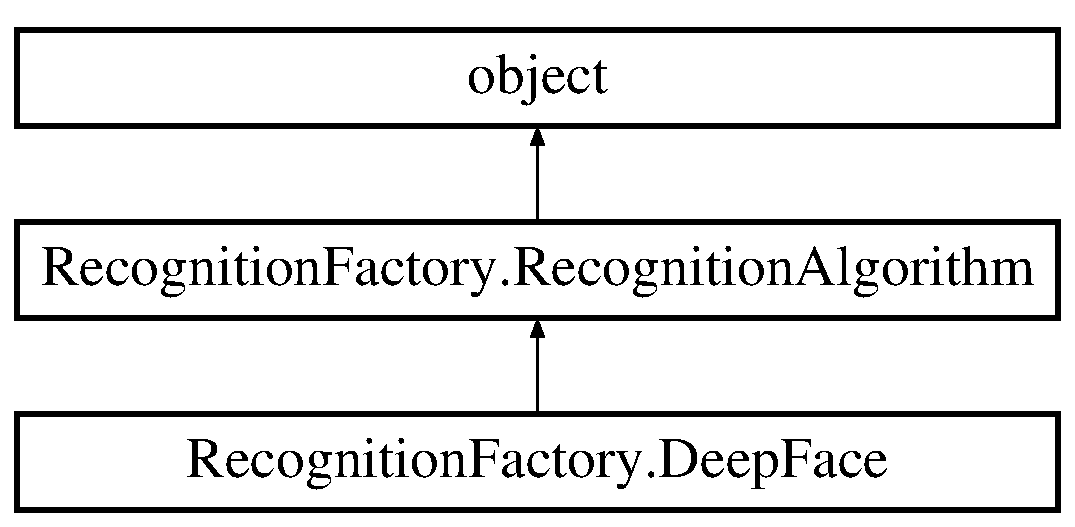
\includegraphics[height=3.000000cm]{classRecognitionFactory_1_1DeepFace}
\end{center}
\end{figure}
\subsection*{Public Member Functions}
\begin{DoxyCompactItemize}
\item 
def {\bfseries \+\_\+\+\_\+init\+\_\+\+\_\+} (self)\hypertarget{classRecognitionFactory_1_1DeepFace_a4c39221f616ceccabdee5fa30b1f1675}{}\label{classRecognitionFactory_1_1DeepFace_a4c39221f616ceccabdee5fa30b1f1675}

\item 
def {\bfseries calc\+\_\+face\+\_\+descriptor} (self, img, bb, landmarks)\hypertarget{classRecognitionFactory_1_1DeepFace_a3f25f9fffd3f0781d4c0ec3105b500c9}{}\label{classRecognitionFactory_1_1DeepFace_a3f25f9fffd3f0781d4c0ec3105b500c9}

\item 
def {\bfseries calc\+\_\+face\+\_\+descriptor\+\_\+aligned\+Image} (self, aligned\+Face, bb)\hypertarget{classRecognitionFactory_1_1DeepFace_ac46fdf7ec084a68ab7b440b58b0efa1d}{}\label{classRecognitionFactory_1_1DeepFace_ac46fdf7ec084a68ab7b440b58b0efa1d}

\item 
def {\bfseries compare} (self, rep1, rep2)\hypertarget{classRecognitionFactory_1_1DeepFace_a71489c980fcab54725c11191d79673fe}{}\label{classRecognitionFactory_1_1DeepFace_a71489c980fcab54725c11191d79673fe}

\end{DoxyCompactItemize}
\subsection*{Public Attributes}
\begin{DoxyCompactItemize}
\item 
{\bfseries modeldir}\hypertarget{classRecognitionFactory_1_1DeepFace_ae9f0b4fa62b5bee40f5284903ae28a79}{}\label{classRecognitionFactory_1_1DeepFace_ae9f0b4fa62b5bee40f5284903ae28a79}

\item 
{\bfseries path\+\_\+to\+\_\+descriptors}\hypertarget{classRecognitionFactory_1_1DeepFace_a1812f707f37da24b92c5b465e9bd72a1}{}\label{classRecognitionFactory_1_1DeepFace_a1812f707f37da24b92c5b465e9bd72a1}

\item 
{\bfseries threshold}\hypertarget{classRecognitionFactory_1_1DeepFace_a99e7d114754ce266408a604327a4e53d}{}\label{classRecognitionFactory_1_1DeepFace_a99e7d114754ce266408a604327a4e53d}

\item 
{\bfseries input\+\_\+image\+\_\+size}\hypertarget{classRecognitionFactory_1_1DeepFace_a094d9b877ae4c19b6a99a6e9c4e3f7df}{}\label{classRecognitionFactory_1_1DeepFace_a094d9b877ae4c19b6a99a6e9c4e3f7df}

\item 
{\bfseries image\+\_\+size}\hypertarget{classRecognitionFactory_1_1DeepFace_afe10131552817f6992ee1da1aca68137}{}\label{classRecognitionFactory_1_1DeepFace_afe10131552817f6992ee1da1aca68137}

\item 
{\bfseries embeddings}\hypertarget{classRecognitionFactory_1_1DeepFace_ad819d9e630129c069b48a9d1108965ca}{}\label{classRecognitionFactory_1_1DeepFace_ad819d9e630129c069b48a9d1108965ca}

\item 
{\bfseries embedding\+\_\+size}\hypertarget{classRecognitionFactory_1_1DeepFace_a936b040d27a005f9a4b8c8e6cfdd5728}{}\label{classRecognitionFactory_1_1DeepFace_a936b040d27a005f9a4b8c8e6cfdd5728}

\item 
{\bfseries images\+\_\+placeholder}\hypertarget{classRecognitionFactory_1_1DeepFace_a43b63b6f56696dd6ac3675ae05f188a4}{}\label{classRecognitionFactory_1_1DeepFace_a43b63b6f56696dd6ac3675ae05f188a4}

\item 
{\bfseries phase\+\_\+train\+\_\+placeholder}\hypertarget{classRecognitionFactory_1_1DeepFace_a283dd13e64bd2970c32ae05a5caeaa44}{}\label{classRecognitionFactory_1_1DeepFace_a283dd13e64bd2970c32ae05a5caeaa44}

\item 
{\bfseries sess}\hypertarget{classRecognitionFactory_1_1DeepFace_ab712a582e7b4198179818ac3f271dc7c}{}\label{classRecognitionFactory_1_1DeepFace_ab712a582e7b4198179818ac3f271dc7c}

\end{DoxyCompactItemize}
\subsection*{Additional Inherited Members}


The documentation for this class was generated from the following file\+:\begin{DoxyCompactItemize}
\item 
py/Recognition\+Factory.\+py\end{DoxyCompactItemize}

\hypertarget{classDetectionFactory_1_1DetectionAlgorithm}{}\section{Detection\+Factory.\+Detection\+Algorithm Class Reference}
\label{classDetectionFactory_1_1DetectionAlgorithm}\index{Detection\+Factory.\+Detection\+Algorithm@{Detection\+Factory.\+Detection\+Algorithm}}
Inheritance diagram for Detection\+Factory.\+Detection\+Algorithm\+:\begin{figure}[H]
\begin{center}
\leavevmode
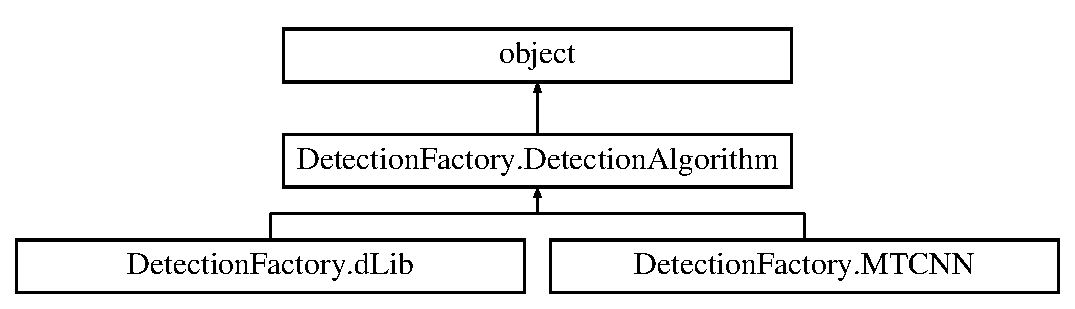
\includegraphics[height=3.000000cm]{classDetectionFactory_1_1DetectionAlgorithm}
\end{center}
\end{figure}
\subsection*{Public Member Functions}
\begin{DoxyCompactItemize}
\item 
def {\bfseries factory} (type)\hypertarget{classDetectionFactory_1_1DetectionAlgorithm_adc7c8e0fd68b235903e55e6f0f13d34a}{}\label{classDetectionFactory_1_1DetectionAlgorithm_adc7c8e0fd68b235903e55e6f0f13d34a}

\end{DoxyCompactItemize}
\subsection*{Static Public Attributes}
\begin{DoxyCompactItemize}
\item 
{\bfseries factory} = staticmethod(factory)\hypertarget{classDetectionFactory_1_1DetectionAlgorithm_aa36820a251819efa6ea1eb7202b270b1}{}\label{classDetectionFactory_1_1DetectionAlgorithm_aa36820a251819efa6ea1eb7202b270b1}

\end{DoxyCompactItemize}


The documentation for this class was generated from the following file\+:\begin{DoxyCompactItemize}
\item 
py/Detection\+Factory.\+py\end{DoxyCompactItemize}

\hypertarget{classRecognitionFactory_1_1dLib}{\section{Recognition\-Factory.\-d\-Lib Class Reference}
\label{classRecognitionFactory_1_1dLib}\index{Recognition\-Factory.\-d\-Lib@{Recognition\-Factory.\-d\-Lib}}
}
Inheritance diagram for Recognition\-Factory.\-d\-Lib\-:\begin{figure}[H]
\begin{center}
\leavevmode
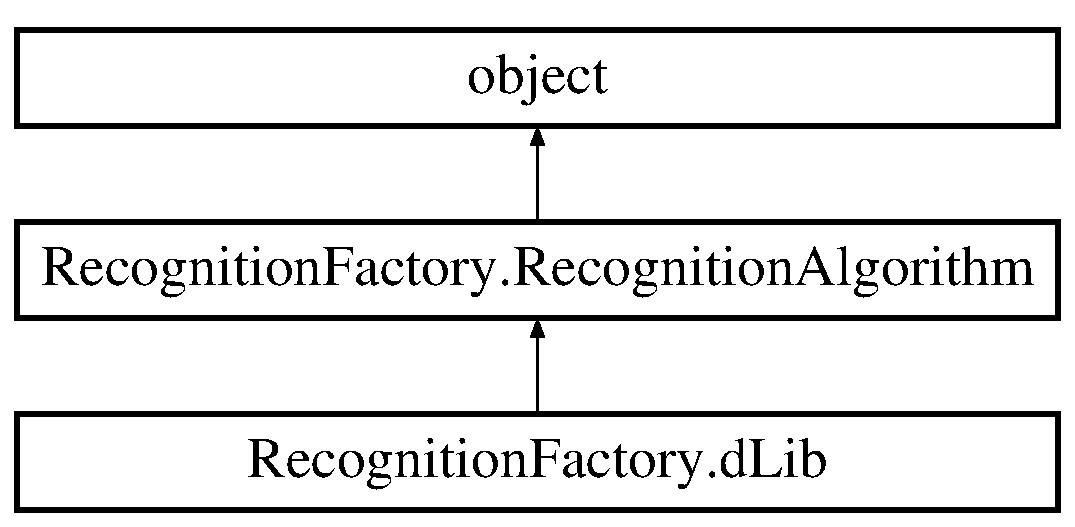
\includegraphics[height=3.000000cm]{classRecognitionFactory_1_1dLib}
\end{center}
\end{figure}
\subsection*{Public Member Functions}
\begin{DoxyCompactItemize}
\item 
def \hyperlink{classRecognitionFactory_1_1dLib_a7bb73498790a1728080d244b168708da}{\-\_\-\-\_\-init\-\_\-\-\_\-}
\begin{DoxyCompactList}\small\item\em Initialization Function. \end{DoxyCompactList}\item 
def \hyperlink{classRecognitionFactory_1_1dLib_acc97bda5d45cea6211c579800157cfff}{calc\-\_\-face\-\_\-descriptor}
\begin{DoxyCompactList}\small\item\em Calculates the face descriptor according to the bounding box and the image given. \end{DoxyCompactList}\item 
def \hyperlink{classRecognitionFactory_1_1dLib_a40973a6daa92cf8801b0e3651a29c83c}{calc\-\_\-face\-\_\-descriptor\-\_\-aligned\-Image}
\begin{DoxyCompactList}\small\item\em Calculates the face descriptor according to an already aligned face. \end{DoxyCompactList}\item 
def \hyperlink{classRecognitionFactory_1_1dLib_adf0aa845ca2d8ff90bb685722dc77f2d}{compare}
\begin{DoxyCompactList}\small\item\em It compares two face descriptors and it will return the similarity between them. \end{DoxyCompactList}\item 
\hypertarget{classRecognitionFactory_1_1dLib_ad428d6482b785537ae2e86113c6ba17d}{def {\bfseries draw}}\label{classRecognitionFactory_1_1dLib_ad428d6482b785537ae2e86113c6ba17d}

\end{DoxyCompactItemize}
\subsection*{Public Attributes}
\begin{DoxyCompactItemize}
\item 
\hypertarget{classRecognitionFactory_1_1dLib_a6957e65ac5c057c4df83936944e779b5}{{\bfseries facerec}}\label{classRecognitionFactory_1_1dLib_a6957e65ac5c057c4df83936944e779b5}

\item 
\hypertarget{classRecognitionFactory_1_1dLib_a0ac95514f25342efc41b1525381e1722}{{\bfseries sp}}\label{classRecognitionFactory_1_1dLib_a0ac95514f25342efc41b1525381e1722}

\item 
\hypertarget{classRecognitionFactory_1_1dLib_a02d8bf3bba4ddfde4d823a5bb3973c27}{{\bfseries path\-\_\-to\-\_\-vectors}}\label{classRecognitionFactory_1_1dLib_a02d8bf3bba4ddfde4d823a5bb3973c27}

\item 
\hypertarget{classRecognitionFactory_1_1dLib_aa3414f96351806052f4343677c34c4da}{{\bfseries threshold}}\label{classRecognitionFactory_1_1dLib_aa3414f96351806052f4343677c34c4da}

\item 
\hypertarget{classRecognitionFactory_1_1dLib_a9505ee9b34f1b5a70390e7fd137b02ee}{{\bfseries aligned\-Face}}\label{classRecognitionFactory_1_1dLib_a9505ee9b34f1b5a70390e7fd137b02ee}

\end{DoxyCompactItemize}
\subsection*{Additional Inherited Members}


\subsection{Constructor \& Destructor Documentation}
\hypertarget{classRecognitionFactory_1_1dLib_a7bb73498790a1728080d244b168708da}{\index{Recognition\-Factory\-::d\-Lib@{Recognition\-Factory\-::d\-Lib}!\-\_\-\-\_\-init\-\_\-\-\_\-@{\-\_\-\-\_\-init\-\_\-\-\_\-}}
\index{\-\_\-\-\_\-init\-\_\-\-\_\-@{\-\_\-\-\_\-init\-\_\-\-\_\-}!RecognitionFactory::dLib@{Recognition\-Factory\-::d\-Lib}}
\subsubsection[{\-\_\-\-\_\-init\-\_\-\-\_\-}]{\setlength{\rightskip}{0pt plus 5cm}def Recognition\-Factory.\-d\-Lib.\-\_\-\-\_\-init\-\_\-\-\_\- (
\begin{DoxyParamCaption}
\item[{}]{self}
\end{DoxyParamCaption}
)}}\label{classRecognitionFactory_1_1dLib_a7bb73498790a1728080d244b168708da}


Initialization Function. 

It will load the models and set the thresholds. 

\subsection{Member Function Documentation}
\hypertarget{classRecognitionFactory_1_1dLib_acc97bda5d45cea6211c579800157cfff}{\index{Recognition\-Factory\-::d\-Lib@{Recognition\-Factory\-::d\-Lib}!calc\-\_\-face\-\_\-descriptor@{calc\-\_\-face\-\_\-descriptor}}
\index{calc\-\_\-face\-\_\-descriptor@{calc\-\_\-face\-\_\-descriptor}!RecognitionFactory::dLib@{Recognition\-Factory\-::d\-Lib}}
\subsubsection[{calc\-\_\-face\-\_\-descriptor}]{\setlength{\rightskip}{0pt plus 5cm}def Recognition\-Factory.\-d\-Lib.\-calc\-\_\-face\-\_\-descriptor (
\begin{DoxyParamCaption}
\item[{}]{self, }
\item[{}]{img, }
\item[{}]{bb, }
\item[{}]{landmarks}
\end{DoxyParamCaption}
)}}\label{classRecognitionFactory_1_1dLib_acc97bda5d45cea6211c579800157cfff}


Calculates the face descriptor according to the bounding box and the image given. 


\begin{DoxyParams}{Parameters}
{\em self} & The object \\
\hline
{\em img} & The image acquired by the camera \\
\hline
{\em bb} & The bounding box of the face detected on the image \\
\hline
{\em landmarks} & The 68 landmarks produced by the function align.\-find\-Landmarks(img, bb)\\
\hline
\end{DoxyParams}
\begin{DoxyReturn}{Returns}
The face descriptor (Array of 128\-D). 
\end{DoxyReturn}
\hypertarget{classRecognitionFactory_1_1dLib_a40973a6daa92cf8801b0e3651a29c83c}{\index{Recognition\-Factory\-::d\-Lib@{Recognition\-Factory\-::d\-Lib}!calc\-\_\-face\-\_\-descriptor\-\_\-aligned\-Image@{calc\-\_\-face\-\_\-descriptor\-\_\-aligned\-Image}}
\index{calc\-\_\-face\-\_\-descriptor\-\_\-aligned\-Image@{calc\-\_\-face\-\_\-descriptor\-\_\-aligned\-Image}!RecognitionFactory::dLib@{Recognition\-Factory\-::d\-Lib}}
\subsubsection[{calc\-\_\-face\-\_\-descriptor\-\_\-aligned\-Image}]{\setlength{\rightskip}{0pt plus 5cm}def Recognition\-Factory.\-d\-Lib.\-calc\-\_\-face\-\_\-descriptor\-\_\-aligned\-Image (
\begin{DoxyParamCaption}
\item[{}]{self, }
\item[{}]{img, }
\item[{}]{bb}
\end{DoxyParamCaption}
)}}\label{classRecognitionFactory_1_1dLib_a40973a6daa92cf8801b0e3651a29c83c}


Calculates the face descriptor according to an already aligned face. 


\begin{DoxyParams}{Parameters}
{\em self} & The object \\
\hline
{\em aligned\-Face} & The aligned face \\
\hline
{\em bb} & The bounding box of the face detected on the image\\
\hline
\end{DoxyParams}
\begin{DoxyReturn}{Returns}
The face descriptor (Array of 128\-D). 
\end{DoxyReturn}
\hypertarget{classRecognitionFactory_1_1dLib_adf0aa845ca2d8ff90bb685722dc77f2d}{\index{Recognition\-Factory\-::d\-Lib@{Recognition\-Factory\-::d\-Lib}!compare@{compare}}
\index{compare@{compare}!RecognitionFactory::dLib@{Recognition\-Factory\-::d\-Lib}}
\subsubsection[{compare}]{\setlength{\rightskip}{0pt plus 5cm}def Recognition\-Factory.\-d\-Lib.\-compare (
\begin{DoxyParamCaption}
\item[{}]{self, }
\item[{}]{face\-\_\-descriptor1, }
\item[{}]{face\-\_\-descriptor2}
\end{DoxyParamCaption}
)}}\label{classRecognitionFactory_1_1dLib_adf0aa845ca2d8ff90bb685722dc77f2d}


It compares two face descriptors and it will return the similarity between them. 


\begin{DoxyParams}{Parameters}
{\em rep1} & First face descriptor \\
\hline
{\em rep2} & Second face descriptor\\
\hline
\end{DoxyParams}
\begin{DoxyReturn}{Returns}
Similairty value 
\end{DoxyReturn}


The documentation for this class was generated from the following file\-:\begin{DoxyCompactItemize}
\item 
py/Recognition\-Factory.\-py\end{DoxyCompactItemize}

\hypertarget{classDetectionFactory_1_1dLib}{}\section{Detection\+Factory.\+d\+Lib Class Reference}
\label{classDetectionFactory_1_1dLib}\index{Detection\+Factory.\+d\+Lib@{Detection\+Factory.\+d\+Lib}}
Inheritance diagram for Detection\+Factory.\+d\+Lib\+:\begin{figure}[H]
\begin{center}
\leavevmode
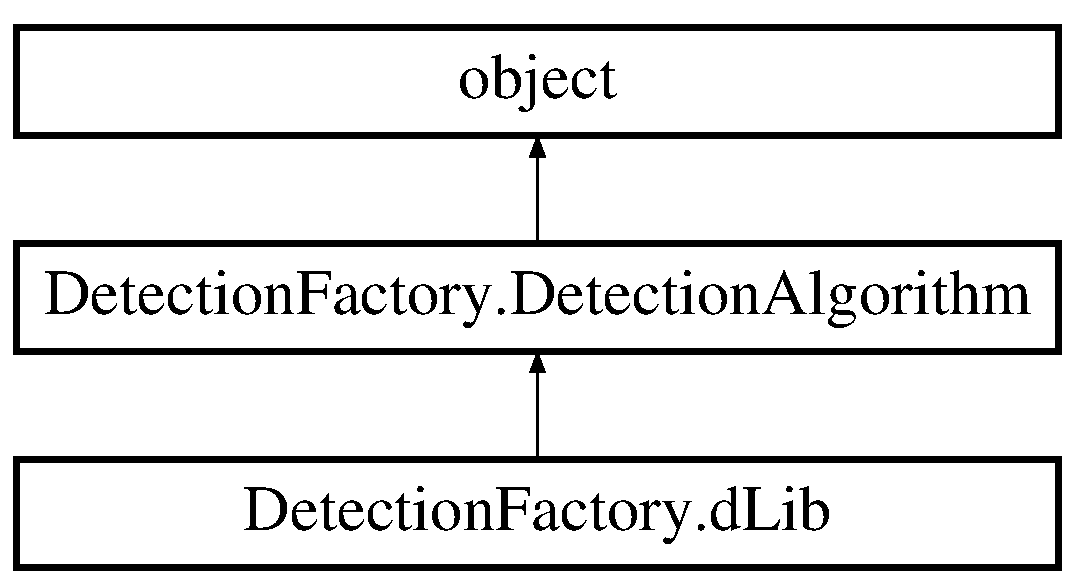
\includegraphics[height=3.000000cm]{classDetectionFactory_1_1dLib}
\end{center}
\end{figure}
\subsection*{Public Member Functions}
\begin{DoxyCompactItemize}
\item 
def {\bfseries \+\_\+\+\_\+init\+\_\+\+\_\+} (self)\hypertarget{classDetectionFactory_1_1dLib_a4fe5ff66e99a50f2e8dc4f5849811ab7}{}\label{classDetectionFactory_1_1dLib_a4fe5ff66e99a50f2e8dc4f5849811ab7}

\item 
def \hyperlink{classDetectionFactory_1_1dLib_af0883422470f60d8a9665b1004ec4acb}{yaw\+\_\+movement} (self, img, bb)
\begin{DoxyCompactList}\small\item\em It will select if the face image is suitable or not to be sent to the verification system according to the yaw movement of the head towards the camera. \end{DoxyCompactList}\item 
def \hyperlink{classDetectionFactory_1_1dLib_a52deb7c6b98fe94459c6521b876b0db9}{blink\+\_\+eyes} (self, img, bb)
\begin{DoxyCompactList}\small\item\em It will select if the face image is suitable or not to be sent to the verification system according to the eyes of the person. \end{DoxyCompactList}\item 
def \hyperlink{classDetectionFactory_1_1dLib_a49e2cf8b779ef27219d8fe20ae8951e5}{face\+\_\+detection} (self, img)
\begin{DoxyCompactList}\small\item\em It will search for the biggest face on the image using dlib\textquotesingle{}s face detection. \end{DoxyCompactList}\end{DoxyCompactItemize}
\subsection*{Public Attributes}
\begin{DoxyCompactItemize}
\item 
{\bfseries align}\hypertarget{classDetectionFactory_1_1dLib_ae29832e1e07a3cd1d8c8b193e70a283d}{}\label{classDetectionFactory_1_1dLib_ae29832e1e07a3cd1d8c8b193e70a283d}

\item 
{\bfseries E\+Y\+E\+\_\+\+T\+I\+P\+N\+O\+S\+E\+\_\+\+E\+YE}\hypertarget{classDetectionFactory_1_1dLib_a5af029331866634c366e650838da5aeb}{}\label{classDetectionFactory_1_1dLib_a5af029331866634c366e650838da5aeb}

\item 
{\bfseries L\+E\+F\+T\+\_\+\+E\+YE}\hypertarget{classDetectionFactory_1_1dLib_a547b03108527d272e4d2594b883ac1cc}{}\label{classDetectionFactory_1_1dLib_a547b03108527d272e4d2594b883ac1cc}

\item 
{\bfseries R\+I\+G\+H\+T\+\_\+\+E\+YE}\hypertarget{classDetectionFactory_1_1dLib_ac3cd4b6a7c5d751105abc3d64ece58ee}{}\label{classDetectionFactory_1_1dLib_ac3cd4b6a7c5d751105abc3d64ece58ee}

\item 
{\bfseries landmarks}\hypertarget{classDetectionFactory_1_1dLib_a611328be1f041fc75dc59d81380b878c}{}\label{classDetectionFactory_1_1dLib_a611328be1f041fc75dc59d81380b878c}

\item 
{\bfseries np\+Landmarks\+\_\+\+Y\+AW}\hypertarget{classDetectionFactory_1_1dLib_a016ab2c80256c30fd2afddbb724f4be5}{}\label{classDetectionFactory_1_1dLib_a016ab2c80256c30fd2afddbb724f4be5}

\item 
{\bfseries img2}\hypertarget{classDetectionFactory_1_1dLib_a8313073c5150f441ca078f148e47cea1}{}\label{classDetectionFactory_1_1dLib_a8313073c5150f441ca078f148e47cea1}

\item 
{\bfseries cc}\hypertarget{classDetectionFactory_1_1dLib_adb115825b8efe01eb788e1bf53c83198}{}\label{classDetectionFactory_1_1dLib_adb115825b8efe01eb788e1bf53c83198}

\item 
{\bfseries bb}\hypertarget{classDetectionFactory_1_1dLib_a78bcd6039095c13740b08c232f610c51}{}\label{classDetectionFactory_1_1dLib_a78bcd6039095c13740b08c232f610c51}

\end{DoxyCompactItemize}
\subsection*{Additional Inherited Members}


\subsection{Member Function Documentation}
\index{Detection\+Factory\+::d\+Lib@{Detection\+Factory\+::d\+Lib}!blink\+\_\+eyes@{blink\+\_\+eyes}}
\index{blink\+\_\+eyes@{blink\+\_\+eyes}!Detection\+Factory\+::d\+Lib@{Detection\+Factory\+::d\+Lib}}
\subsubsection[{\texorpdfstring{blink\+\_\+eyes(self, img, bb)}{blink_eyes(self, img, bb)}}]{\setlength{\rightskip}{0pt plus 5cm}def Detection\+Factory.\+d\+Lib.\+blink\+\_\+eyes (
\begin{DoxyParamCaption}
\item[{}]{self, }
\item[{}]{img, }
\item[{}]{bb}
\end{DoxyParamCaption}
)}\hypertarget{classDetectionFactory_1_1dLib_a52deb7c6b98fe94459c6521b876b0db9}{}\label{classDetectionFactory_1_1dLib_a52deb7c6b98fe94459c6521b876b0db9}


It will select if the face image is suitable or not to be sent to the verification system according to the eyes of the person. 

If the person has his/her eyes closed then the image will not be used for the verification system.


\begin{DoxyParams}{Parameters}
{\em img} & Image acquired by the camera \\
\hline
{\em bb} & Bounding box that delineates the biggest face found on the image\\
\hline
\end{DoxyParams}

\begin{DoxyRetVals}{Return values}
{\em True} & if the face image is suitable to be sent \\
\hline
{\em False} & if not \\
\hline
\end{DoxyRetVals}
\index{Detection\+Factory\+::d\+Lib@{Detection\+Factory\+::d\+Lib}!face\+\_\+detection@{face\+\_\+detection}}
\index{face\+\_\+detection@{face\+\_\+detection}!Detection\+Factory\+::d\+Lib@{Detection\+Factory\+::d\+Lib}}
\subsubsection[{\texorpdfstring{face\+\_\+detection(self, img)}{face_detection(self, img)}}]{\setlength{\rightskip}{0pt plus 5cm}def Detection\+Factory.\+d\+Lib.\+face\+\_\+detection (
\begin{DoxyParamCaption}
\item[{}]{self, }
\item[{}]{img}
\end{DoxyParamCaption}
)}\hypertarget{classDetectionFactory_1_1dLib_a49e2cf8b779ef27219d8fe20ae8951e5}{}\label{classDetectionFactory_1_1dLib_a49e2cf8b779ef27219d8fe20ae8951e5}


It will search for the biggest face on the image using dlib\textquotesingle{}s face detection. 


\begin{DoxyParams}{Parameters}
{\em img} & Image acquired by the camera\\
\hline
\end{DoxyParams}

\begin{DoxyRetVals}{Return values}
{\em True} & if there is a face detected \\
\hline
{\em False} & if not \\
\hline
\end{DoxyRetVals}
\index{Detection\+Factory\+::d\+Lib@{Detection\+Factory\+::d\+Lib}!yaw\+\_\+movement@{yaw\+\_\+movement}}
\index{yaw\+\_\+movement@{yaw\+\_\+movement}!Detection\+Factory\+::d\+Lib@{Detection\+Factory\+::d\+Lib}}
\subsubsection[{\texorpdfstring{yaw\+\_\+movement(self, img, bb)}{yaw_movement(self, img, bb)}}]{\setlength{\rightskip}{0pt plus 5cm}def Detection\+Factory.\+d\+Lib.\+yaw\+\_\+movement (
\begin{DoxyParamCaption}
\item[{}]{self, }
\item[{}]{img, }
\item[{}]{bb}
\end{DoxyParamCaption}
)}\hypertarget{classDetectionFactory_1_1dLib_af0883422470f60d8a9665b1004ec4acb}{}\label{classDetectionFactory_1_1dLib_af0883422470f60d8a9665b1004ec4acb}


It will select if the face image is suitable or not to be sent to the verification system according to the yaw movement of the head towards the camera. 


\begin{DoxyParams}{Parameters}
{\em img} & Image acquired by the camera \\
\hline
{\em bb} & Bounding box that delineates the biggest face found on the image\\
\hline
\end{DoxyParams}

\begin{DoxyRetVals}{Return values}
{\em True} & if the face image is suitable to be sent \\
\hline
{\em False} & if not \\
\hline
\end{DoxyRetVals}


The documentation for this class was generated from the following file\+:\begin{DoxyCompactItemize}
\item 
py/Detection\+Factory.\+py\end{DoxyCompactItemize}

\hypertarget{classfacenet_1_1ImageClass}{}\section{facenet.\+Image\+Class Class Reference}
\label{classfacenet_1_1ImageClass}\index{facenet.\+Image\+Class@{facenet.\+Image\+Class}}
\subsection*{Public Member Functions}
\begin{DoxyCompactItemize}
\item 
def {\bfseries \+\_\+\+\_\+init\+\_\+\+\_\+} (self, name, image\+\_\+paths)\hypertarget{classfacenet_1_1ImageClass_a9cd9daa35d2f22f9d3cf61404f0fa93b}{}\label{classfacenet_1_1ImageClass_a9cd9daa35d2f22f9d3cf61404f0fa93b}

\item 
def {\bfseries \+\_\+\+\_\+str\+\_\+\+\_\+} (self)\hypertarget{classfacenet_1_1ImageClass_a51a4385e652bbbd415c21d68d94d16d6}{}\label{classfacenet_1_1ImageClass_a51a4385e652bbbd415c21d68d94d16d6}

\item 
def {\bfseries \+\_\+\+\_\+len\+\_\+\+\_\+} (self)\hypertarget{classfacenet_1_1ImageClass_a0fef51f010849335f39d39015bcc6ae3}{}\label{classfacenet_1_1ImageClass_a0fef51f010849335f39d39015bcc6ae3}

\end{DoxyCompactItemize}
\subsection*{Public Attributes}
\begin{DoxyCompactItemize}
\item 
{\bfseries name}\hypertarget{classfacenet_1_1ImageClass_a9be0826646711d9200a31b8c5cfcf1c2}{}\label{classfacenet_1_1ImageClass_a9be0826646711d9200a31b8c5cfcf1c2}

\item 
{\bfseries image\+\_\+paths}\hypertarget{classfacenet_1_1ImageClass_afd647167440b4ab86847ae2954771a69}{}\label{classfacenet_1_1ImageClass_afd647167440b4ab86847ae2954771a69}

\end{DoxyCompactItemize}


The documentation for this class was generated from the following file\+:\begin{DoxyCompactItemize}
\item 
py/facenet.\+py\end{DoxyCompactItemize}

\hypertarget{classDetectionFactory_1_1MTCNN}{}\section{Detection\+Factory.\+M\+T\+C\+NN Class Reference}
\label{classDetectionFactory_1_1MTCNN}\index{Detection\+Factory.\+M\+T\+C\+NN@{Detection\+Factory.\+M\+T\+C\+NN}}
Inheritance diagram for Detection\+Factory.\+M\+T\+C\+NN\+:\begin{figure}[H]
\begin{center}
\leavevmode
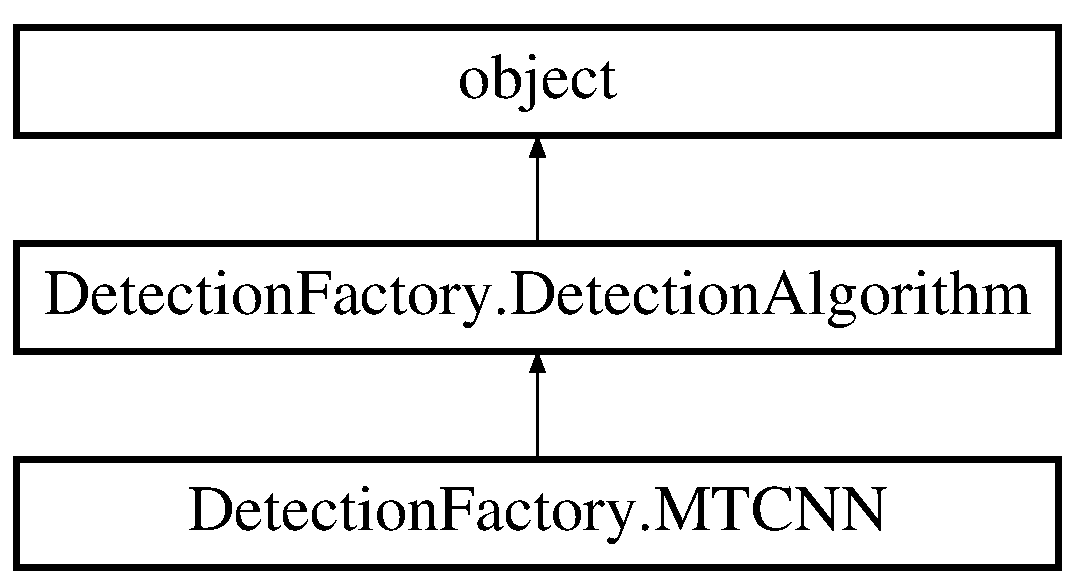
\includegraphics[height=3.000000cm]{classDetectionFactory_1_1MTCNN}
\end{center}
\end{figure}
\subsection*{Public Member Functions}
\begin{DoxyCompactItemize}
\item 
def {\bfseries \+\_\+\+\_\+init\+\_\+\+\_\+} (self)\hypertarget{classDetectionFactory_1_1MTCNN_abb5e3f6589b98423f5ea579a303c999b}{}\label{classDetectionFactory_1_1MTCNN_abb5e3f6589b98423f5ea579a303c999b}

\item 
def \hyperlink{classDetectionFactory_1_1MTCNN_ac7d884cb82b4ac91212453121238e641}{yaw\+\_\+movement} (self, img, bb)
\begin{DoxyCompactList}\small\item\em It will select if the face image is suitable or not to be sent to the verification system according to the yaw movement of the head towards the camera. \end{DoxyCompactList}\item 
def \hyperlink{classDetectionFactory_1_1MTCNN_a879b84b1ec40bdd68775e7f2368bb856}{blink\+\_\+eyes} (self, img, bb)
\begin{DoxyCompactList}\small\item\em It will select if the face image is suitable or not to be sent to the verification system according to the eyes of the person. \end{DoxyCompactList}\item 
def \hyperlink{classDetectionFactory_1_1MTCNN_a10083feb0513bee3bdffca54ca1596be}{face\+\_\+detection} (self, img)
\begin{DoxyCompactList}\small\item\em It will search for the biggest face on the image using dlib\textquotesingle{}s face detection. \end{DoxyCompactList}\end{DoxyCompactItemize}
\subsection*{Public Attributes}
\begin{DoxyCompactItemize}
\item 
{\bfseries onet}\hypertarget{classDetectionFactory_1_1MTCNN_a620b2a799a7152753f5b1e2450fb4c95}{}\label{classDetectionFactory_1_1MTCNN_a620b2a799a7152753f5b1e2450fb4c95}

\item 
{\bfseries minsize}\hypertarget{classDetectionFactory_1_1MTCNN_a88a63fe4097b7472254b5e4c27c08136}{}\label{classDetectionFactory_1_1MTCNN_a88a63fe4097b7472254b5e4c27c08136}

\item 
{\bfseries threshold}\hypertarget{classDetectionFactory_1_1MTCNN_aa03ad85cc768388c5b62b74bd63d1359}{}\label{classDetectionFactory_1_1MTCNN_aa03ad85cc768388c5b62b74bd63d1359}

\item 
{\bfseries factor}\hypertarget{classDetectionFactory_1_1MTCNN_a1dc564bd588f6af67eb8ef512df433ab}{}\label{classDetectionFactory_1_1MTCNN_a1dc564bd588f6af67eb8ef512df433ab}

\item 
{\bfseries margin}\hypertarget{classDetectionFactory_1_1MTCNN_a09ecd3174676e45de708ca99ecbe64b7}{}\label{classDetectionFactory_1_1MTCNN_a09ecd3174676e45de708ca99ecbe64b7}

\item 
{\bfseries image\+\_\+size}\hypertarget{classDetectionFactory_1_1MTCNN_af61041c4a7ca9791e88f33ee3ea71e67}{}\label{classDetectionFactory_1_1MTCNN_af61041c4a7ca9791e88f33ee3ea71e67}

\item 
{\bfseries img2}\hypertarget{classDetectionFactory_1_1MTCNN_ae87e713438cdb63a191a69d28aec497b}{}\label{classDetectionFactory_1_1MTCNN_ae87e713438cdb63a191a69d28aec497b}

\item 
{\bfseries cc}\hypertarget{classDetectionFactory_1_1MTCNN_a676877a356d9b222c7afe1d5ba515dd1}{}\label{classDetectionFactory_1_1MTCNN_a676877a356d9b222c7afe1d5ba515dd1}

\item 
{\bfseries landmarks}\hypertarget{classDetectionFactory_1_1MTCNN_a31d4a96842c6285659c64e6239dcda22}{}\label{classDetectionFactory_1_1MTCNN_a31d4a96842c6285659c64e6239dcda22}

\item 
{\bfseries bb}\hypertarget{classDetectionFactory_1_1MTCNN_abcc415a7a422ca85fcec23cc426a27e4}{}\label{classDetectionFactory_1_1MTCNN_abcc415a7a422ca85fcec23cc426a27e4}

\end{DoxyCompactItemize}
\subsection*{Additional Inherited Members}


\subsection{Member Function Documentation}
\index{Detection\+Factory\+::\+M\+T\+C\+NN@{Detection\+Factory\+::\+M\+T\+C\+NN}!blink\+\_\+eyes@{blink\+\_\+eyes}}
\index{blink\+\_\+eyes@{blink\+\_\+eyes}!Detection\+Factory\+::\+M\+T\+C\+NN@{Detection\+Factory\+::\+M\+T\+C\+NN}}
\subsubsection[{\texorpdfstring{blink\+\_\+eyes(self, img, bb)}{blink_eyes(self, img, bb)}}]{\setlength{\rightskip}{0pt plus 5cm}def Detection\+Factory.\+M\+T\+C\+N\+N.\+blink\+\_\+eyes (
\begin{DoxyParamCaption}
\item[{}]{self, }
\item[{}]{img, }
\item[{}]{bb}
\end{DoxyParamCaption}
)}\hypertarget{classDetectionFactory_1_1MTCNN_a879b84b1ec40bdd68775e7f2368bb856}{}\label{classDetectionFactory_1_1MTCNN_a879b84b1ec40bdd68775e7f2368bb856}


It will select if the face image is suitable or not to be sent to the verification system according to the eyes of the person. 

If the person has his/her eyes closed then the image will not be used for the verification system.


\begin{DoxyParams}{Parameters}
{\em img} & Image acquired by the camera \\
\hline
{\em bb} & Bounding box that delineates the biggest face found on the image\\
\hline
\end{DoxyParams}

\begin{DoxyRetVals}{Return values}
{\em True} & if the face image is suitable to be sent \\
\hline
{\em False} & if not \\
\hline
\end{DoxyRetVals}
\index{Detection\+Factory\+::\+M\+T\+C\+NN@{Detection\+Factory\+::\+M\+T\+C\+NN}!face\+\_\+detection@{face\+\_\+detection}}
\index{face\+\_\+detection@{face\+\_\+detection}!Detection\+Factory\+::\+M\+T\+C\+NN@{Detection\+Factory\+::\+M\+T\+C\+NN}}
\subsubsection[{\texorpdfstring{face\+\_\+detection(self, img)}{face_detection(self, img)}}]{\setlength{\rightskip}{0pt plus 5cm}def Detection\+Factory.\+M\+T\+C\+N\+N.\+face\+\_\+detection (
\begin{DoxyParamCaption}
\item[{}]{self, }
\item[{}]{img}
\end{DoxyParamCaption}
)}\hypertarget{classDetectionFactory_1_1MTCNN_a10083feb0513bee3bdffca54ca1596be}{}\label{classDetectionFactory_1_1MTCNN_a10083feb0513bee3bdffca54ca1596be}


It will search for the biggest face on the image using dlib\textquotesingle{}s face detection. 


\begin{DoxyParams}{Parameters}
{\em img} & Image acquired by the camera\\
\hline
\end{DoxyParams}

\begin{DoxyRetVals}{Return values}
{\em True} & if there is a face detected \\
\hline
{\em False} & if not \\
\hline
\end{DoxyRetVals}
\index{Detection\+Factory\+::\+M\+T\+C\+NN@{Detection\+Factory\+::\+M\+T\+C\+NN}!yaw\+\_\+movement@{yaw\+\_\+movement}}
\index{yaw\+\_\+movement@{yaw\+\_\+movement}!Detection\+Factory\+::\+M\+T\+C\+NN@{Detection\+Factory\+::\+M\+T\+C\+NN}}
\subsubsection[{\texorpdfstring{yaw\+\_\+movement(self, img, bb)}{yaw_movement(self, img, bb)}}]{\setlength{\rightskip}{0pt plus 5cm}def Detection\+Factory.\+M\+T\+C\+N\+N.\+yaw\+\_\+movement (
\begin{DoxyParamCaption}
\item[{}]{self, }
\item[{}]{img, }
\item[{}]{bb}
\end{DoxyParamCaption}
)}\hypertarget{classDetectionFactory_1_1MTCNN_ac7d884cb82b4ac91212453121238e641}{}\label{classDetectionFactory_1_1MTCNN_ac7d884cb82b4ac91212453121238e641}


It will select if the face image is suitable or not to be sent to the verification system according to the yaw movement of the head towards the camera. 


\begin{DoxyParams}{Parameters}
{\em img} & Image acquired by the camera \\
\hline
{\em bb} & Bounding box that delineates the biggest face found on the image\\
\hline
\end{DoxyParams}

\begin{DoxyRetVals}{Return values}
{\em True} & if the face image is suitable to be sent \\
\hline
{\em False} & if not \\
\hline
\end{DoxyRetVals}


The documentation for this class was generated from the following file\+:\begin{DoxyCompactItemize}
\item 
py/Detection\+Factory.\+py\end{DoxyCompactItemize}

\hypertarget{classdetect__face_1_1Network}{}\section{detect\+\_\+face.\+Network Class Reference}
\label{classdetect__face_1_1Network}\index{detect\+\_\+face.\+Network@{detect\+\_\+face.\+Network}}
Inheritance diagram for detect\+\_\+face.\+Network\+:\begin{figure}[H]
\begin{center}
\leavevmode
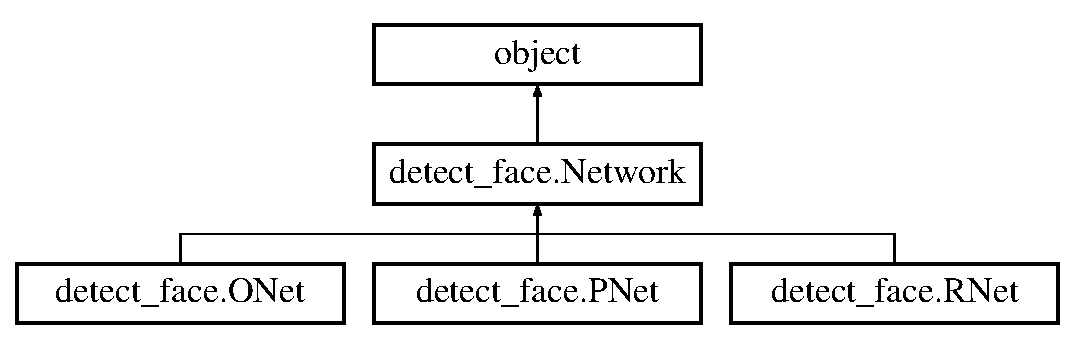
\includegraphics[height=3.000000cm]{classdetect__face_1_1Network}
\end{center}
\end{figure}
\subsection*{Public Member Functions}
\begin{DoxyCompactItemize}
\item 
def {\bfseries \+\_\+\+\_\+init\+\_\+\+\_\+} (self, inputs, trainable=True)\hypertarget{classdetect__face_1_1Network_a69f8b4b309d9f5402ccb86f73a34d807}{}\label{classdetect__face_1_1Network_a69f8b4b309d9f5402ccb86f73a34d807}

\item 
def \hyperlink{classdetect__face_1_1Network_ac19da11c9d5136399bee1c5b2468be79}{setup} (self)
\item 
def \hyperlink{classdetect__face_1_1Network_a26cf4112c7a92cc8d03e74e690c6831d}{load} (self, data\+\_\+path, session, ignore\+\_\+missing=False)
\item 
def \hyperlink{classdetect__face_1_1Network_a810da0416a4cd84e83015d89131d4389}{feed} (self, args)
\item 
def \hyperlink{classdetect__face_1_1Network_a4a6eb7a13da3620697a64f7a974242e8}{get\+\_\+output} (self)
\item 
def \hyperlink{classdetect__face_1_1Network_aa6ee08c64a7f8a75ac13a485a8ed3374}{get\+\_\+unique\+\_\+name} (self, prefix)
\item 
def \hyperlink{classdetect__face_1_1Network_a4ee4b07dc43c4092f4c1b63d89296057}{make\+\_\+var} (self, name, shape)
\item 
def \hyperlink{classdetect__face_1_1Network_a8f407ab687e3a91324e0b54b9011672a}{validate\+\_\+padding} (self, padding)
\item 
def {\bfseries conv} (self, inp, k\+\_\+h, k\+\_\+w, c\+\_\+o, s\+\_\+h, s\+\_\+w, name, relu=True, padding=\textquotesingle{}S\+A\+ME\textquotesingle{}, group=1, biased=True)\hypertarget{classdetect__face_1_1Network_a3f5730dec069754ebd608eedf81669ed}{}\label{classdetect__face_1_1Network_a3f5730dec069754ebd608eedf81669ed}

\item 
def {\bfseries prelu} (self, inp, name)\hypertarget{classdetect__face_1_1Network_a6ab3ca1c0884bacf4bc4fd608ed766fd}{}\label{classdetect__face_1_1Network_a6ab3ca1c0884bacf4bc4fd608ed766fd}

\item 
def {\bfseries max\+\_\+pool} (self, inp, k\+\_\+h, k\+\_\+w, s\+\_\+h, s\+\_\+w, name, padding=\textquotesingle{}S\+A\+ME\textquotesingle{})\hypertarget{classdetect__face_1_1Network_a1ef26550a38cce16c26d5b8858a6864f}{}\label{classdetect__face_1_1Network_a1ef26550a38cce16c26d5b8858a6864f}

\item 
def {\bfseries fc} (self, inp, num\+\_\+out, name, relu=True)\hypertarget{classdetect__face_1_1Network_a5450f5698fd15318d12dbd18b4b9ef72}{}\label{classdetect__face_1_1Network_a5450f5698fd15318d12dbd18b4b9ef72}

\item 
def {\bfseries softmax} (self, target, axis, name=None)\hypertarget{classdetect__face_1_1Network_a7376e5641477584f8819d5d9e5043eb8}{}\label{classdetect__face_1_1Network_a7376e5641477584f8819d5d9e5043eb8}

\end{DoxyCompactItemize}
\subsection*{Public Attributes}
\begin{DoxyCompactItemize}
\item 
{\bfseries inputs}\hypertarget{classdetect__face_1_1Network_a869d691efce01f7d4d70f159a93a1f90}{}\label{classdetect__face_1_1Network_a869d691efce01f7d4d70f159a93a1f90}

\item 
{\bfseries terminals}\hypertarget{classdetect__face_1_1Network_a827c4a5dbba9486bbbe439cf66b200db}{}\label{classdetect__face_1_1Network_a827c4a5dbba9486bbbe439cf66b200db}

\item 
{\bfseries layers}\hypertarget{classdetect__face_1_1Network_ae6cf34012bc82d05b239ead904527aeb}{}\label{classdetect__face_1_1Network_ae6cf34012bc82d05b239ead904527aeb}

\item 
{\bfseries trainable}\hypertarget{classdetect__face_1_1Network_a9f44e04ca2ba3fd708e28c1d1d340350}{}\label{classdetect__face_1_1Network_a9f44e04ca2ba3fd708e28c1d1d340350}

\end{DoxyCompactItemize}


\subsection{Member Function Documentation}
\index{detect\+\_\+face\+::\+Network@{detect\+\_\+face\+::\+Network}!feed@{feed}}
\index{feed@{feed}!detect\+\_\+face\+::\+Network@{detect\+\_\+face\+::\+Network}}
\subsubsection[{\texorpdfstring{feed(self, args)}{feed(self, args)}}]{\setlength{\rightskip}{0pt plus 5cm}def detect\+\_\+face.\+Network.\+feed (
\begin{DoxyParamCaption}
\item[{}]{self, }
\item[{}]{args}
\end{DoxyParamCaption}
)}\hypertarget{classdetect__face_1_1Network_a810da0416a4cd84e83015d89131d4389}{}\label{classdetect__face_1_1Network_a810da0416a4cd84e83015d89131d4389}
\begin{DoxyVerb}Set the input(s) for the next operation by replacing the terminal nodes.
The arguments can be either layer names or the actual layers.
\end{DoxyVerb}
 \index{detect\+\_\+face\+::\+Network@{detect\+\_\+face\+::\+Network}!get\+\_\+output@{get\+\_\+output}}
\index{get\+\_\+output@{get\+\_\+output}!detect\+\_\+face\+::\+Network@{detect\+\_\+face\+::\+Network}}
\subsubsection[{\texorpdfstring{get\+\_\+output(self)}{get_output(self)}}]{\setlength{\rightskip}{0pt plus 5cm}def detect\+\_\+face.\+Network.\+get\+\_\+output (
\begin{DoxyParamCaption}
\item[{}]{self}
\end{DoxyParamCaption}
)}\hypertarget{classdetect__face_1_1Network_a4a6eb7a13da3620697a64f7a974242e8}{}\label{classdetect__face_1_1Network_a4a6eb7a13da3620697a64f7a974242e8}
\begin{DoxyVerb}Returns the current network output.\end{DoxyVerb}
 \index{detect\+\_\+face\+::\+Network@{detect\+\_\+face\+::\+Network}!get\+\_\+unique\+\_\+name@{get\+\_\+unique\+\_\+name}}
\index{get\+\_\+unique\+\_\+name@{get\+\_\+unique\+\_\+name}!detect\+\_\+face\+::\+Network@{detect\+\_\+face\+::\+Network}}
\subsubsection[{\texorpdfstring{get\+\_\+unique\+\_\+name(self, prefix)}{get_unique_name(self, prefix)}}]{\setlength{\rightskip}{0pt plus 5cm}def detect\+\_\+face.\+Network.\+get\+\_\+unique\+\_\+name (
\begin{DoxyParamCaption}
\item[{}]{self, }
\item[{}]{prefix}
\end{DoxyParamCaption}
)}\hypertarget{classdetect__face_1_1Network_aa6ee08c64a7f8a75ac13a485a8ed3374}{}\label{classdetect__face_1_1Network_aa6ee08c64a7f8a75ac13a485a8ed3374}
\begin{DoxyVerb}Returns an index-suffixed unique name for the given prefix.
This is used for auto-generating layer names based on the type-prefix.
\end{DoxyVerb}
 \index{detect\+\_\+face\+::\+Network@{detect\+\_\+face\+::\+Network}!load@{load}}
\index{load@{load}!detect\+\_\+face\+::\+Network@{detect\+\_\+face\+::\+Network}}
\subsubsection[{\texorpdfstring{load(self, data\+\_\+path, session, ignore\+\_\+missing=\+False)}{load(self, data_path, session, ignore_missing=False)}}]{\setlength{\rightskip}{0pt plus 5cm}def detect\+\_\+face.\+Network.\+load (
\begin{DoxyParamCaption}
\item[{}]{self, }
\item[{}]{data\+\_\+path, }
\item[{}]{session, }
\item[{}]{ignore\+\_\+missing = {\ttfamily False}}
\end{DoxyParamCaption}
)}\hypertarget{classdetect__face_1_1Network_a26cf4112c7a92cc8d03e74e690c6831d}{}\label{classdetect__face_1_1Network_a26cf4112c7a92cc8d03e74e690c6831d}
\begin{DoxyVerb}Load network weights.
data_path: The path to the numpy-serialized network weights
session: The current TensorFlow session
ignore_missing: If true, serialized weights for missing layers are ignored.
\end{DoxyVerb}
 \index{detect\+\_\+face\+::\+Network@{detect\+\_\+face\+::\+Network}!make\+\_\+var@{make\+\_\+var}}
\index{make\+\_\+var@{make\+\_\+var}!detect\+\_\+face\+::\+Network@{detect\+\_\+face\+::\+Network}}
\subsubsection[{\texorpdfstring{make\+\_\+var(self, name, shape)}{make_var(self, name, shape)}}]{\setlength{\rightskip}{0pt plus 5cm}def detect\+\_\+face.\+Network.\+make\+\_\+var (
\begin{DoxyParamCaption}
\item[{}]{self, }
\item[{}]{name, }
\item[{}]{shape}
\end{DoxyParamCaption}
)}\hypertarget{classdetect__face_1_1Network_a4ee4b07dc43c4092f4c1b63d89296057}{}\label{classdetect__face_1_1Network_a4ee4b07dc43c4092f4c1b63d89296057}
\begin{DoxyVerb}Creates a new TensorFlow variable.\end{DoxyVerb}
 \index{detect\+\_\+face\+::\+Network@{detect\+\_\+face\+::\+Network}!setup@{setup}}
\index{setup@{setup}!detect\+\_\+face\+::\+Network@{detect\+\_\+face\+::\+Network}}
\subsubsection[{\texorpdfstring{setup(self)}{setup(self)}}]{\setlength{\rightskip}{0pt plus 5cm}def detect\+\_\+face.\+Network.\+setup (
\begin{DoxyParamCaption}
\item[{}]{self}
\end{DoxyParamCaption}
)}\hypertarget{classdetect__face_1_1Network_ac19da11c9d5136399bee1c5b2468be79}{}\label{classdetect__face_1_1Network_ac19da11c9d5136399bee1c5b2468be79}
\begin{DoxyVerb}Construct the network. \end{DoxyVerb}
 \index{detect\+\_\+face\+::\+Network@{detect\+\_\+face\+::\+Network}!validate\+\_\+padding@{validate\+\_\+padding}}
\index{validate\+\_\+padding@{validate\+\_\+padding}!detect\+\_\+face\+::\+Network@{detect\+\_\+face\+::\+Network}}
\subsubsection[{\texorpdfstring{validate\+\_\+padding(self, padding)}{validate_padding(self, padding)}}]{\setlength{\rightskip}{0pt plus 5cm}def detect\+\_\+face.\+Network.\+validate\+\_\+padding (
\begin{DoxyParamCaption}
\item[{}]{self, }
\item[{}]{padding}
\end{DoxyParamCaption}
)}\hypertarget{classdetect__face_1_1Network_a8f407ab687e3a91324e0b54b9011672a}{}\label{classdetect__face_1_1Network_a8f407ab687e3a91324e0b54b9011672a}
\begin{DoxyVerb}Verifies that the padding is one of the supported ones.\end{DoxyVerb}
 

The documentation for this class was generated from the following file\+:\begin{DoxyCompactItemize}
\item 
py/detect\+\_\+face.\+py\end{DoxyCompactItemize}

\hypertarget{classdetect__face_1_1ONet}{}\section{detect\+\_\+face.\+O\+Net Class Reference}
\label{classdetect__face_1_1ONet}\index{detect\+\_\+face.\+O\+Net@{detect\+\_\+face.\+O\+Net}}
Inheritance diagram for detect\+\_\+face.\+O\+Net\+:\begin{figure}[H]
\begin{center}
\leavevmode
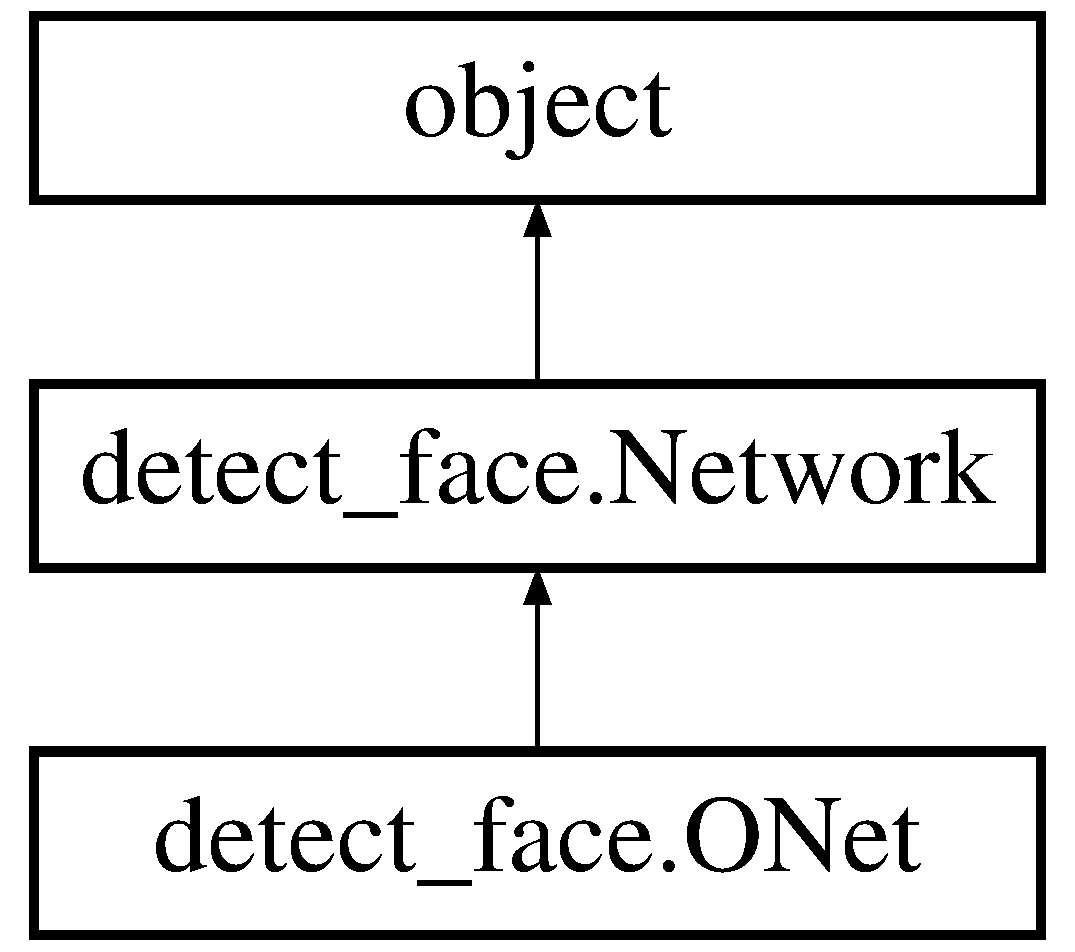
\includegraphics[height=3.000000cm]{classdetect__face_1_1ONet}
\end{center}
\end{figure}
\subsection*{Public Member Functions}
\begin{DoxyCompactItemize}
\item 
def {\bfseries setup} (self)\hypertarget{classdetect__face_1_1ONet_a3ea3e2c1fbff5de5806bb9c54c817116}{}\label{classdetect__face_1_1ONet_a3ea3e2c1fbff5de5806bb9c54c817116}

\end{DoxyCompactItemize}
\subsection*{Additional Inherited Members}


The documentation for this class was generated from the following file\+:\begin{DoxyCompactItemize}
\item 
py/detect\+\_\+face.\+py\end{DoxyCompactItemize}

\hypertarget{classRecognitionFactory_1_1OpenFace}{}\section{Recognition\+Factory.\+Open\+Face Class Reference}
\label{classRecognitionFactory_1_1OpenFace}\index{Recognition\+Factory.\+Open\+Face@{Recognition\+Factory.\+Open\+Face}}
Inheritance diagram for Recognition\+Factory.\+Open\+Face\+:\begin{figure}[H]
\begin{center}
\leavevmode
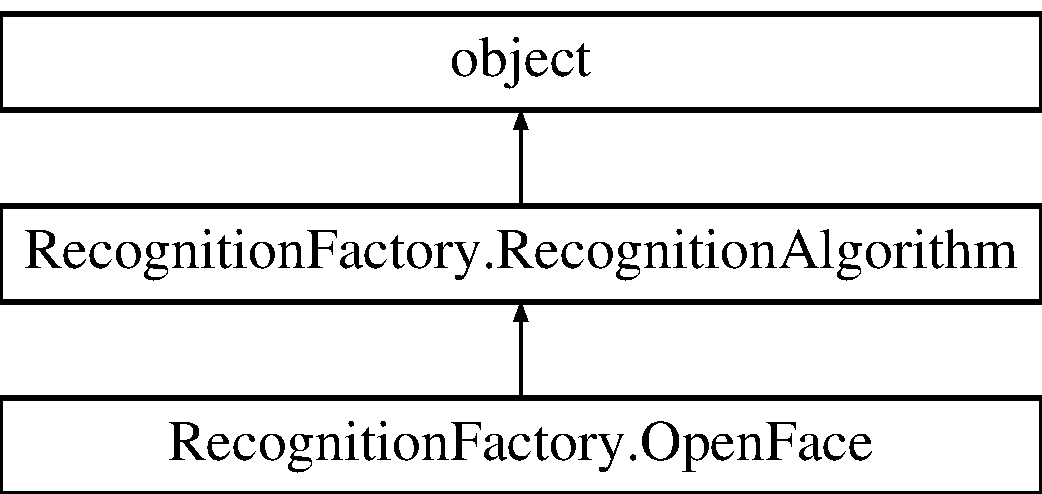
\includegraphics[height=3.000000cm]{classRecognitionFactory_1_1OpenFace}
\end{center}
\end{figure}
\subsection*{Public Member Functions}
\begin{DoxyCompactItemize}
\item 
def {\bfseries \+\_\+\+\_\+init\+\_\+\+\_\+} (self)\hypertarget{classRecognitionFactory_1_1OpenFace_a555a6f98154c13480cd0221bbb616cdc}{}\label{classRecognitionFactory_1_1OpenFace_a555a6f98154c13480cd0221bbb616cdc}

\item 
def \hyperlink{classRecognitionFactory_1_1OpenFace_a836912f1319b9a6b433439514b411e85}{calc\+\_\+face\+\_\+descriptor} (self, img, bb, landmarks)
\begin{DoxyCompactList}\small\item\em According to the image given, it will align the face, apply the preprocessing technique (if aplicable) and then forward through the neural network. \end{DoxyCompactList}\item 
def \hyperlink{classRecognitionFactory_1_1OpenFace_aaf88498d63d98982547f19ee314e5bba}{calc\+\_\+face\+\_\+descriptor\+\_\+aligned\+Image} (self, aligned\+Face, bb)
\begin{DoxyCompactList}\small\item\em According to the face image given, it will apply the preprocessing technique (if aplicable) and then forward through the neural network. \end{DoxyCompactList}\item 
def \hyperlink{classRecognitionFactory_1_1OpenFace_afa0790d2f75b5191265048c584dbb858}{compare} (self, rep1, rep2)
\begin{DoxyCompactList}\small\item\em Given two face descriptors it subtract one to the other and then calculates the norm of the vector. \end{DoxyCompactList}\end{DoxyCompactItemize}
\subsection*{Public Attributes}
\begin{DoxyCompactItemize}
\item 
{\bfseries align}\hypertarget{classRecognitionFactory_1_1OpenFace_a1c901bdf709de3d7e1b40093af926974}{}\label{classRecognitionFactory_1_1OpenFace_a1c901bdf709de3d7e1b40093af926974}

\item 
{\bfseries openface\+Model\+Dir}\hypertarget{classRecognitionFactory_1_1OpenFace_a1ee73330a23fce8a6ca41231d778ec91}{}\label{classRecognitionFactory_1_1OpenFace_a1ee73330a23fce8a6ca41231d778ec91}

\item 
{\bfseries path\+\_\+to\+\_\+descriptors}\hypertarget{classRecognitionFactory_1_1OpenFace_acaa350f52e5e1a71b2d6643403ec1af1}{}\label{classRecognitionFactory_1_1OpenFace_acaa350f52e5e1a71b2d6643403ec1af1}

\item 
{\bfseries net}\hypertarget{classRecognitionFactory_1_1OpenFace_a4cd893ba8a2c3882481901c1093c3ae3}{}\label{classRecognitionFactory_1_1OpenFace_a4cd893ba8a2c3882481901c1093c3ae3}

\item 
{\bfseries threshold}\hypertarget{classRecognitionFactory_1_1OpenFace_a334cc50444b6906a8c08ec658c8f5438}{}\label{classRecognitionFactory_1_1OpenFace_a334cc50444b6906a8c08ec658c8f5438}

\item 
{\bfseries aligned\+Face}\hypertarget{classRecognitionFactory_1_1OpenFace_a1acaa386b19695644e18eab416f390ee}{}\label{classRecognitionFactory_1_1OpenFace_a1acaa386b19695644e18eab416f390ee}

\end{DoxyCompactItemize}
\subsection*{Additional Inherited Members}


\subsection{Member Function Documentation}
\index{Recognition\+Factory\+::\+Open\+Face@{Recognition\+Factory\+::\+Open\+Face}!calc\+\_\+face\+\_\+descriptor@{calc\+\_\+face\+\_\+descriptor}}
\index{calc\+\_\+face\+\_\+descriptor@{calc\+\_\+face\+\_\+descriptor}!Recognition\+Factory\+::\+Open\+Face@{Recognition\+Factory\+::\+Open\+Face}}
\subsubsection[{\texorpdfstring{calc\+\_\+face\+\_\+descriptor(self, img, bb, landmarks)}{calc_face_descriptor(self, img, bb, landmarks)}}]{\setlength{\rightskip}{0pt plus 5cm}def Recognition\+Factory.\+Open\+Face.\+calc\+\_\+face\+\_\+descriptor (
\begin{DoxyParamCaption}
\item[{}]{self, }
\item[{}]{img, }
\item[{}]{bb, }
\item[{}]{landmarks}
\end{DoxyParamCaption}
)}\hypertarget{classRecognitionFactory_1_1OpenFace_a836912f1319b9a6b433439514b411e85}{}\label{classRecognitionFactory_1_1OpenFace_a836912f1319b9a6b433439514b411e85}


According to the image given, it will align the face, apply the preprocessing technique (if aplicable) and then forward through the neural network. 


\begin{DoxyParams}{Parameters}
{\em img} & Image acquired by the camera \\
\hline
{\em bb} & Bounding box that delineates the biggest face found on the image\\
\hline
\end{DoxyParams}

\begin{DoxyRetVals}{Return values}
{\em The} & face descriptor \\
\hline
\end{DoxyRetVals}
\index{Recognition\+Factory\+::\+Open\+Face@{Recognition\+Factory\+::\+Open\+Face}!calc\+\_\+face\+\_\+descriptor\+\_\+aligned\+Image@{calc\+\_\+face\+\_\+descriptor\+\_\+aligned\+Image}}
\index{calc\+\_\+face\+\_\+descriptor\+\_\+aligned\+Image@{calc\+\_\+face\+\_\+descriptor\+\_\+aligned\+Image}!Recognition\+Factory\+::\+Open\+Face@{Recognition\+Factory\+::\+Open\+Face}}
\subsubsection[{\texorpdfstring{calc\+\_\+face\+\_\+descriptor\+\_\+aligned\+Image(self, aligned\+Face, bb)}{calc_face_descriptor_alignedImage(self, alignedFace, bb)}}]{\setlength{\rightskip}{0pt plus 5cm}def Recognition\+Factory.\+Open\+Face.\+calc\+\_\+face\+\_\+descriptor\+\_\+aligned\+Image (
\begin{DoxyParamCaption}
\item[{}]{self, }
\item[{}]{aligned\+Face, }
\item[{}]{bb}
\end{DoxyParamCaption}
)}\hypertarget{classRecognitionFactory_1_1OpenFace_aaf88498d63d98982547f19ee314e5bba}{}\label{classRecognitionFactory_1_1OpenFace_aaf88498d63d98982547f19ee314e5bba}


According to the face image given, it will apply the preprocessing technique (if aplicable) and then forward through the neural network. 


\begin{DoxyParams}{Parameters}
{\em img} & Face image gave by the face detector \\
\hline
{\em bb} & Not used, can be anything\\
\hline
\end{DoxyParams}

\begin{DoxyRetVals}{Return values}
{\em The} & face descriptor \\
\hline
\end{DoxyRetVals}
\index{Recognition\+Factory\+::\+Open\+Face@{Recognition\+Factory\+::\+Open\+Face}!compare@{compare}}
\index{compare@{compare}!Recognition\+Factory\+::\+Open\+Face@{Recognition\+Factory\+::\+Open\+Face}}
\subsubsection[{\texorpdfstring{compare(self, rep1, rep2)}{compare(self, rep1, rep2)}}]{\setlength{\rightskip}{0pt plus 5cm}def Recognition\+Factory.\+Open\+Face.\+compare (
\begin{DoxyParamCaption}
\item[{}]{self, }
\item[{}]{rep1, }
\item[{}]{rep2}
\end{DoxyParamCaption}
)}\hypertarget{classRecognitionFactory_1_1OpenFace_afa0790d2f75b5191265048c584dbb858}{}\label{classRecognitionFactory_1_1OpenFace_afa0790d2f75b5191265048c584dbb858}


Given two face descriptors it subtract one to the other and then calculates the norm of the vector. 

This is also called the similarity between two vectors. It is usally made on the face verification process and facetracking. The higher the value the more likely that it is a different person.


\begin{DoxyParams}{Parameters}
{\em face\+\_\+descriptor1} & Face image gave by the face detector \\
\hline
{\em face\+\_\+descriptor2} & Bounding box that delineates the biggest face found on the image (in this case is the face image dimensions)\\
\hline
\end{DoxyParams}

\begin{DoxyRetVals}{Return values}
{\em Value} & of similarity between vectors \\
\hline
\end{DoxyRetVals}


The documentation for this class was generated from the following file\+:\begin{DoxyCompactItemize}
\item 
py/Recognition\+Factory.\+py\end{DoxyCompactItemize}

\hypertarget{classdetect__face_1_1PNet}{}\section{detect\+\_\+face.\+P\+Net Class Reference}
\label{classdetect__face_1_1PNet}\index{detect\+\_\+face.\+P\+Net@{detect\+\_\+face.\+P\+Net}}
Inheritance diagram for detect\+\_\+face.\+P\+Net\+:\begin{figure}[H]
\begin{center}
\leavevmode
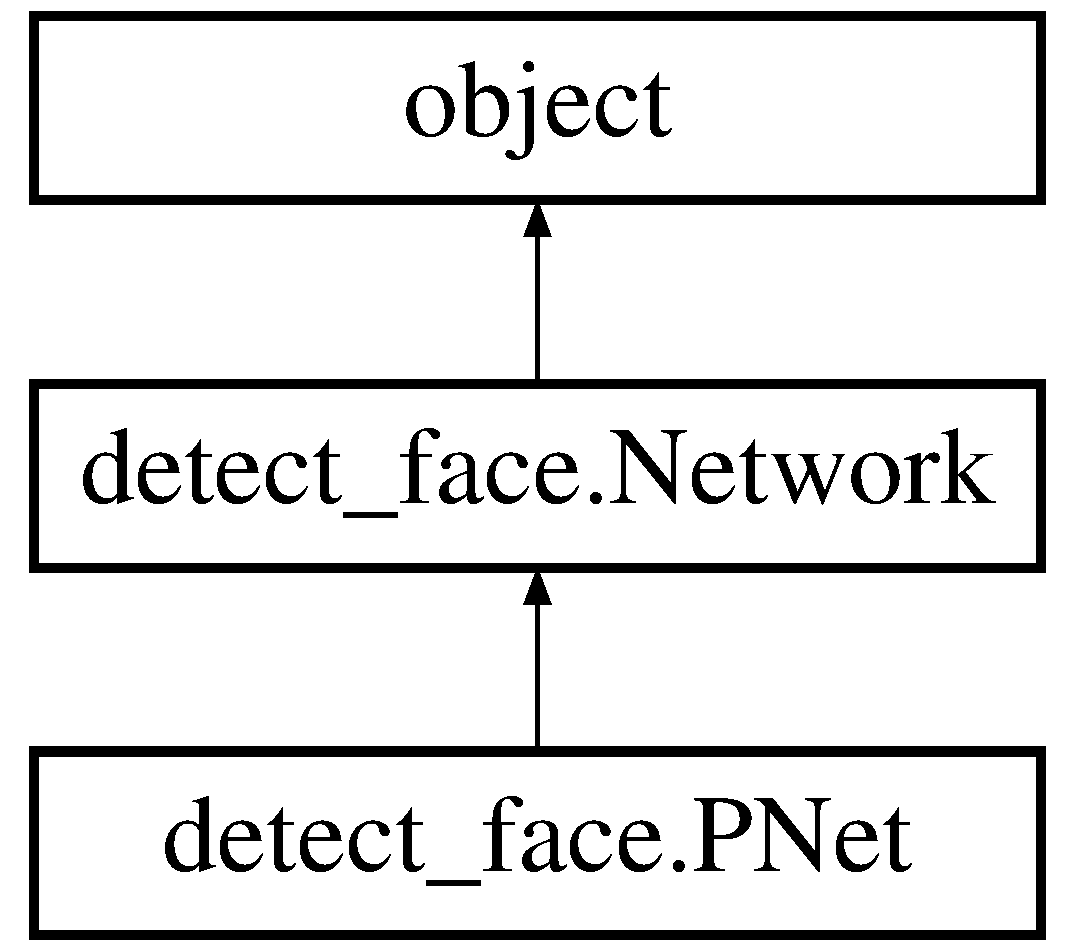
\includegraphics[height=3.000000cm]{classdetect__face_1_1PNet}
\end{center}
\end{figure}
\subsection*{Public Member Functions}
\begin{DoxyCompactItemize}
\item 
def {\bfseries setup} (self)\hypertarget{classdetect__face_1_1PNet_a971a1b62952a9c7c6b926516536f244e}{}\label{classdetect__face_1_1PNet_a971a1b62952a9c7c6b926516536f244e}

\end{DoxyCompactItemize}
\subsection*{Additional Inherited Members}


The documentation for this class was generated from the following file\+:\begin{DoxyCompactItemize}
\item 
py/detect\+\_\+face.\+py\end{DoxyCompactItemize}

\hypertarget{classRecognitionFactory_1_1RecognitionAlgorithm}{\section{Recognition\-Factory.\-Recognition\-Algorithm Class Reference}
\label{classRecognitionFactory_1_1RecognitionAlgorithm}\index{Recognition\-Factory.\-Recognition\-Algorithm@{Recognition\-Factory.\-Recognition\-Algorithm}}
}


Recognition factory to choose which algorithm will be used.  


Inheritance diagram for Recognition\-Factory.\-Recognition\-Algorithm\-:\begin{figure}[H]
\begin{center}
\leavevmode
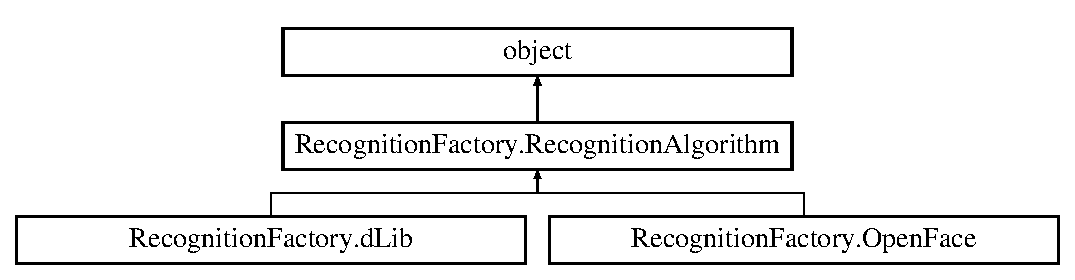
\includegraphics[height=3.000000cm]{classRecognitionFactory_1_1RecognitionAlgorithm}
\end{center}
\end{figure}
\subsection*{Public Member Functions}
\begin{DoxyCompactItemize}
\item 
\hypertarget{classRecognitionFactory_1_1RecognitionAlgorithm_acc15c6c8c13e74e4fa5848141b3a98bb}{def {\bfseries factory}}\label{classRecognitionFactory_1_1RecognitionAlgorithm_acc15c6c8c13e74e4fa5848141b3a98bb}

\end{DoxyCompactItemize}
\subsection*{Static Public Attributes}
\begin{DoxyCompactItemize}
\item 
\hypertarget{classRecognitionFactory_1_1RecognitionAlgorithm_a9d948cf769252cf8bdc07639332203d3}{tuple {\bfseries factory} = staticmethod(factory)}\label{classRecognitionFactory_1_1RecognitionAlgorithm_a9d948cf769252cf8bdc07639332203d3}

\end{DoxyCompactItemize}


\subsection{Detailed Description}
Recognition factory to choose which algorithm will be used. 

(\hyperlink{classRecognitionFactory_1_1dLib}{d\-Lib} or \hyperlink{classRecognitionFactory_1_1OpenFace}{Open\-Face}). 

The documentation for this class was generated from the following file\-:\begin{DoxyCompactItemize}
\item 
py/Recognition\-Factory.\-py\end{DoxyCompactItemize}

\hypertarget{classdetect__face_1_1RNet}{}\section{detect\+\_\+face.\+R\+Net Class Reference}
\label{classdetect__face_1_1RNet}\index{detect\+\_\+face.\+R\+Net@{detect\+\_\+face.\+R\+Net}}
Inheritance diagram for detect\+\_\+face.\+R\+Net\+:\begin{figure}[H]
\begin{center}
\leavevmode
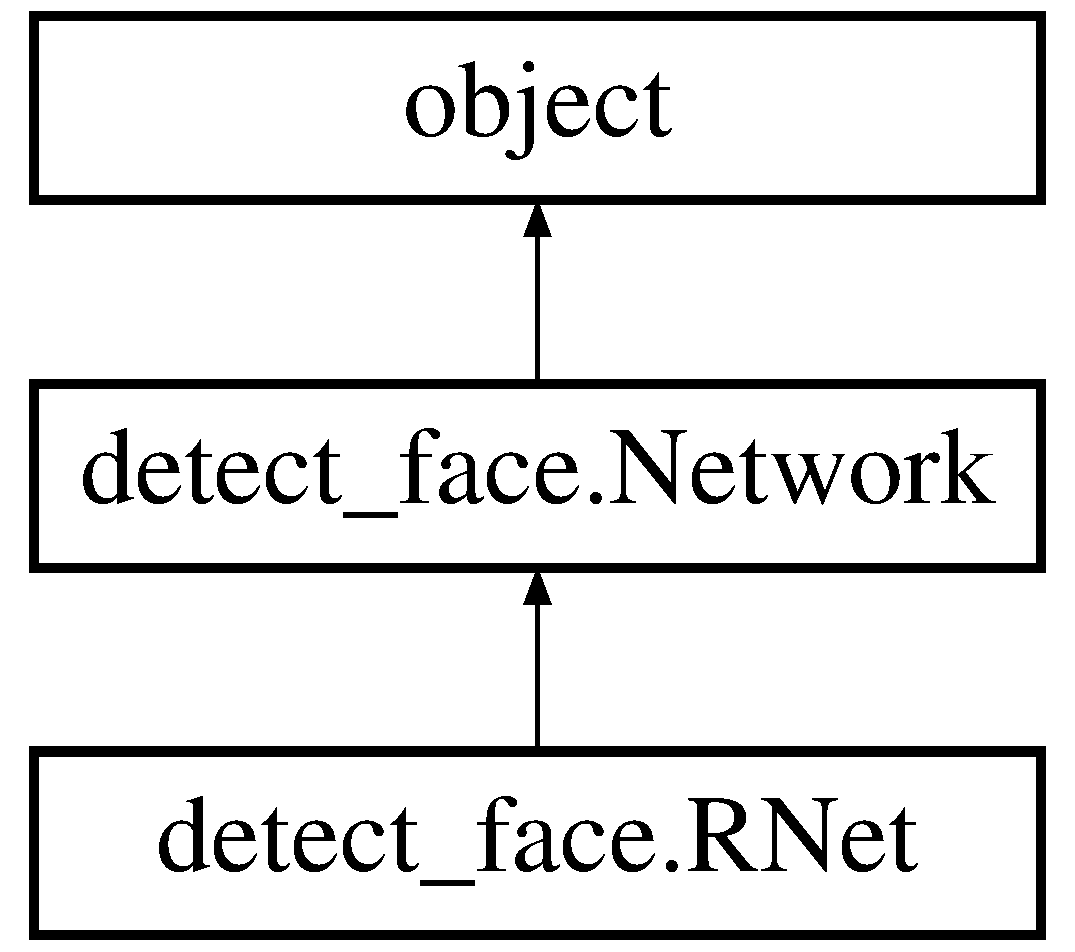
\includegraphics[height=3.000000cm]{classdetect__face_1_1RNet}
\end{center}
\end{figure}
\subsection*{Public Member Functions}
\begin{DoxyCompactItemize}
\item 
def {\bfseries setup} (self)\hypertarget{classdetect__face_1_1RNet_a0e76e16f5e899ed0dc92123676e44410}{}\label{classdetect__face_1_1RNet_a0e76e16f5e899ed0dc92123676e44410}

\end{DoxyCompactItemize}
\subsection*{Additional Inherited Members}


The documentation for this class was generated from the following file\+:\begin{DoxyCompactItemize}
\item 
py/detect\+\_\+face.\+py\end{DoxyCompactItemize}

%--- End generated contents ---

% Index
\backmatter
\newpage
\phantomsection
\clearemptydoublepage
\addcontentsline{toc}{chapter}{Index}
\printindex

\end{document}
